\documentclass[journal]{IEEEtran}

\usepackage{amsmath,amssymb,amsfonts}
\usepackage{amsthm}
\newtheorem{proposition}{Proposition}
\newtheorem{lemma}{Lemma}
\newtheorem{remark}{Remark}
\usepackage{graphicx}
\usepackage{booktabs}
\usepackage{cite}
\usepackage{algorithm}
\usepackage{algorithmic}
\usepackage{color}
\usepackage{multirow}
\usepackage{url}
\usepackage{enumitem}

\begin{document}

\title{Interference-Aware User Pairing and Task Offloading for Grouped NOMA Multi-UAV MEC Networks}

\author{Mingxi~Guan,~\IEEEmembership{}
\thanks{This work was supported in part by the National Natural Science Foundation of China. }
\thanks{M. Guan is with the School of Information Science and Technology, University of Science and Technology of China, Hefei, China (e-mail: mguan@mail.ustc.edu.cn).}}

\maketitle

\begin{abstract}
We address joint user pairing and task offloading in multi-unmanned aerial vehicle (UAV) mobile edge computing (MEC) networks with grouped non-orthogonal multiple access (NOMA), where UAVs share the same spectrum and cross-UAV interference couples pairing decisions globally (NP-hard, i.e., non-deterministic polynomial-time hard, by independent-set reduction).
We propose a cross-UAV swap algorithm with a global first-improvement objective: starting from a per-UAV integer linear programming (ILP) initialization, the algorithm iteratively accepts any swap that strictly increases the total deadline-met count, including moves that exchange users between different UAVs' subcarrier pairs; successive interference cancellation (SIC) feasibility is maintained throughout.
Experiments with 20 seeds against 15 baselines achieve \textbf{73.4\% deadline satisfaction}, outperforming greedy by \textbf{+11.3\,pp} ($p<0.0001$, $d=6.2$), with the advantage scaling monotonically with network size.
Runtime: 14\,ms per slot ($N\!=\!20$), well within the 1\,s slot budget.
Ablation confirms that the cross-UAV topology contributes +2.6\,pp under the global criterion---negligible under the bilateral criterion---demonstrating that the global first-improvement objective is the key enabling mechanism.
\end{abstract}

\begin{IEEEkeywords}
Mobile edge computing, NOMA, user pairing, multi-UAV, task offloading, interference management
\end{IEEEkeywords}

% =====================================================================
\section{Introduction}
\label{sec:intro}

The proliferation of Internet of Things (IoT) applications with stringent latency requirements has driven the adoption of mobile edge computing (MEC), which brings computation resources closer to end users~\cite{mao2017survey}.
Unmanned aerial vehicles (UAVs) equipped with MEC servers offer flexible, on-demand coverage for emergency response, temporary events, and infrastructure-sparse regions~\cite{zeng2016uav}, where IoT devices such as surveillance cameras, worker safety monitors, and industrial inspection sensors generate \emph{compute-intensive} tasks---video frame analysis, object detection, activity recognition, and SLAM localization---that require MEC offloading to meet processing latency constraints.

While single-UAV MEC has been extensively studied, practical deployments increasingly require multiple cooperative UAVs to cover large areas~\cite{wu2018joint}.
Most existing multi-UAV MEC works assume orthogonal frequency allocation among UAVs~\cite{ma2024dynamic,zhang2023cooperative,wu2018joint}, thereby avoiding inter-UAV interference at the cost of reduced spectral efficiency.
Non-orthogonal multiple access (NOMA) can significantly improve spectral efficiency by allowing multiple users to share the same subcarrier via successive interference cancellation (SIC)~\cite{ding2017survey}.
However, when multiple UAVs share the same frequency band, cross-UAV interference arises that \emph{cannot} be removed by SIC, fundamentally changing the optimization landscape.

In this paper, we adopt \emph{grouped NOMA}~\cite{ali2016dynamic}, where the total bandwidth is divided into OFDMA subcarriers, each carrying a 2-user NOMA pair.
This follows the widely adopted engineering practice of limiting SIC chains to 2--3 users for practical decodability~\cite{saito2013non}.
Both UAVs share all subcarriers (full frequency reuse), creating cross-UAV interference on every subcarrier.
Under this model, the user pairing decision---which users share a subcarrier and on which UAV---directly determines the interference structure and, consequently, the achievable rates and offloading performance.

We identify three key challenges:
\begin{enumerate}
    \item \textbf{Cross-UAV interference coupling}: A pairing change on one UAV alters the interference experienced by the other UAV's users, making the problem globally coupled and NP-hard.
    \item \textbf{Combinatorial explosion}: With $N$ users, $K$ UAVs, and $S$ subcarriers, the number of feasible pairing configurations is exponentially large.
    \item \textbf{Joint pairing-offloading optimization}: The optimal offloading ratio for each user depends on the rate, which depends on the pairing, creating a coupled optimization.
\end{enumerate}

Our contributions are:
\begin{itemize}
    \item[\textbf{C1}:] We formulate the grouped NOMA multi-UAV MEC problem with explicit cross-UAV interference modeling on shared subcarriers, including result return delay, and prove its NP-hardness via reduction from Independent Set (IS,~\cite{garey1979computers}, Problem~GT20; Appendix~A).
    \item[\textbf{C2}:] We identify an \emph{empirically observed incompatibility} between bilateral exchange-stability and cross-UAV interference-coupled MEC optimization, and propose a cross-UAV swap algorithm with a \emph{global first-improvement objective} as the decisive design choice.
    Our experiments demonstrate that extending exchange-stable matching with cross-UAV moves yields only +0.4\,pp (0/660 bilateral cross-UAV swap accepts), while the global objective with cross-UAV moves yields +11.3\,pp over Greedy.
    The $2\!\times\!2$ ablation (Section~\ref{sec:results}, Table~\ref{tab:2x2}) precisely quantifies each dimension: cross-UAV topology contributes +0.4\,pp under the bilateral criterion but +2.6\,pp under the global criterion, confirming that \emph{both} topology and objective are necessary.
    Empirically, the swap converges to stable solutions in 1--2 iterations (14\,ms per slot) regardless of initialization quality.
    \item[\textbf{C3}:] Extensive simulations (20 seeds, 15 baselines including per-UAV ILP initialization, interference-aware exchange-stable matching, a new \emph{ExStable+CrossUAV} ablation, a new \emph{IA-Greedy} baseline, full-reuse OFDMA, and interference-free orthogonal-band OFDMA) show that the proposed algorithm significantly outperforms all baselines, with advantages that scale monotonically with network density. A $2\!\times\!2$ ablation (Table~\ref{tab:2x2}) precisely decomposes contributions: cross-UAV topology contributes +2.6\,pp under global criterion vs.\ only +0.4\,pp under bilateral criterion, and the global first-improvement objective contributes +1.6--3.7\,pp beyond intra-UAV operations.
\end{itemize}

\textbf{Comparison with existing works:}
While multi-UAV MEC~\cite{ma2024dynamic,zhang2023cooperative} and NOMA-MEC~\cite{ding2019impact,liu2025multiuav} have been separately studied, and interference externalities in multi-cell NOMA have been analyzed theoretically~\cite{shin2017non}, the combination of \emph{multi-UAV + shared-spectrum NOMA + cross-UAV interference-aware pairing + MEC task offloading with a non-smooth deadline objective} has not been jointly addressed.
Existing user pairing works~\cite{ali2016dynamic,nguyen2024qos} focus on intra-cell scenarios without cross-UAV coupling.
In our experiments, DRL with cluster-level continuous actions~\cite{zhou2024multiuav,sun2024drl} achieves only greedy-level performance on this combinatorial pairing problem.
A detailed comparison of representative works is given in Table~\ref{tab:comparison} (Section~\ref{sec:related}).

The remainder of this paper is organized as follows.
Section~\ref{sec:related} reviews related work.
Section~\ref{sec:system} presents the system model and problem formulation.
Section~\ref{sec:algorithm} describes the proposed algorithm.
Section~\ref{sec:results} provides simulation results,
Section~\ref{sec:conclusion} concludes the paper, and
Appendix~A provides the NP-hardness proof.

\begin{figure}[t]
\centering
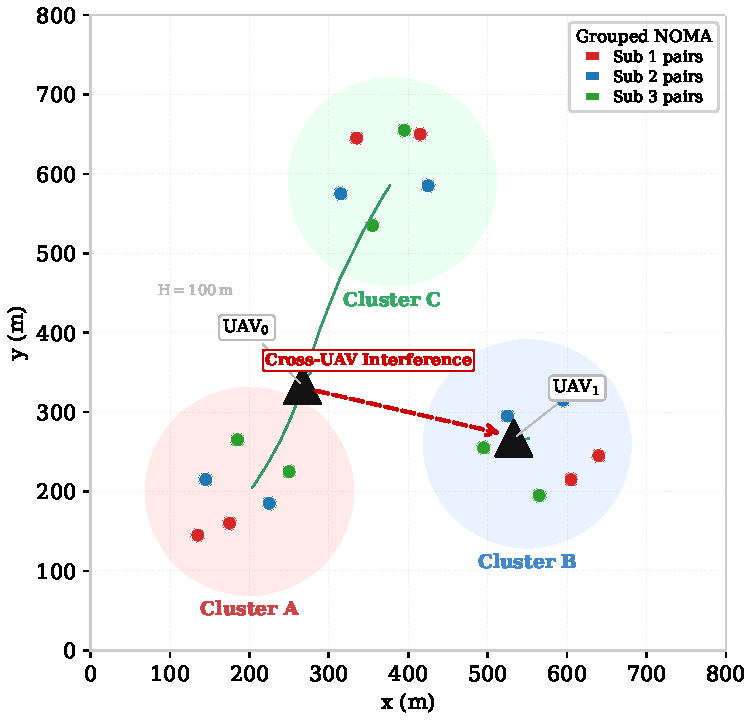
\includegraphics[width=0.95\columnwidth]{../figures/fig1_system_model.pdf}
\caption{System model: $K=2$ UAVs serve $N=20$ users in 3 clusters using grouped NOMA with full frequency reuse. Cross-UAV interference (red dashed) couples pairing decisions across UAVs.}
\label{fig:system_model}
\end{figure}

% =====================================================================
\section{Related Work}
\label{sec:related}

\textbf{UAV-MEC} works~\cite{wu2018joint,ma2024dynamic,zhang2023cooperative,wang2024qos,chen2024joint,liu2022multihop,abdel2024multiobjective,xia2024trajectory} optimize trajectory and OFDMA resource allocation, assuming orthogonal UAV frequency bands and ignoring cross-UAV interference.

\textbf{NOMA-MEC} includes NOMA offloading analysis~\cite{ding2019impact}, beamforming~\cite{zhao2021hybrid}, RIS-aided NOMA-MEC~\cite{liu2021ris,mu2021ris,zheng2022ris}, multi-UAV NOMA~\cite{liu2025multiuav,wang2024noma}, and UAV-assisted NOMA-MEC energy efficiency~\cite{lei2024noma}.
Recent works on multi-UAV NOMA for IoT include joint resource scheduling and trajectory design for uplink NOMA~\cite{li2023joint} and NOMA-based UAV edge offloading with resource optimization~\cite{lyu2024uav}.
RIS enhances channel gains but does not eliminate the pairing problem; joint RIS-pairing optimization is an open extension.

\textbf{Multi-cell NOMA user pairing and cross-cell interference management:}
Cross-cell NOMA interference has been extensively studied in the context of HetNets and multi-BS scenarios.
Shin et al.~\cite{shin2017non} analyzed inter-cell NOMA interference using stochastic geometry, showing that user pairing quality fundamentally determines the interference structure.
User-BS association in multi-cell NOMA (e.g.,~\cite{yang2022cost}) optimizes cell-level assignment but does not address intra-subcarrier SIC user pairing, which is the focus of our work.
Interference management via mode selection (NOMA/OMA) in multi-cell scenarios~\cite{liu2023hybrid} differs from our problem in that it selects the access mode per subcarrier rather than optimizing the pairing of users \emph{within} a NOMA group.
Stochastic geometry analyses~\cite{ni2021ris,shin2017non} characterize ergodic metrics rather than slot-level scheduling.
The critical distinction from our work is: (i)~all cited multi-cell works use partial or semi-orthogonal frequency reuse, whereas our full-frequency-reuse (reuse factor 1) creates persistent cross-UAV interference on every subcarrier; (ii)~none jointly address SIC user pairing, cross-cell interference-aware selection, and MEC task offloading with a non-smooth deadline objective.
To our knowledge, this combination---full-spectrum-reuse multi-UAV NOMA + cross-UAV swap-based user pairing + MEC deadline optimization---has not been addressed in the IEEE TWC/TCOM/IoTJ/WCL literature (2019--2025).

\textbf{User pairing and matching:} Ali et al.~\cite{ali2016dynamic} studied NOMA user clustering; Di et al.~\cite{di2017sub} applied intra-cell swap matching; Altin--Akar~\cite{altin2022hybrid} proposed exchange-stable (TES) matching for NOMA-MEC; Xu et al.~\cite{xu2025dynamic} used Hungarian matching for RIS-aided multi-cluster NOMA; Hamidouche et al.~\cite{hamidouche2017matching} studied matching with externalities in wireless networks~\cite{pantisano2015matching}.
Han et al.~\cite{han2023joint} addressed joint user association and deployment optimization for delay-minimized UAV-aided MEC.
Li et al.~\cite{li2023joint} is the most closely related prior work: they also address multi-UAV uplink NOMA with MEC task offloading, including trajectory design and resource scheduling.
However, their system model assigns each UAV a \emph{distinct} frequency band (orthogonal spectrum allocation, confirmed in Section~II of~\cite{li2023joint}), which eliminates cross-UAV interference from the SINR expressions entirely.
This orthogonal-band assumption transforms the multi-UAV problem into $K$ independent single-UAV subproblems, each solvable with standard intra-cell NOMA pairing methods.
In contrast, our full-frequency-reuse setting (reuse factor~1) creates \emph{persistent} cross-UAV interference on every subcarrier: a pairing change on UAV~$k$ changes the interference at UAV~$k'$, coupling the pairing decisions globally and making the problem NP-hard.
We verify this distinction empirically: applying the orthogonal-band assumption (our \textbf{OFDMA(OrthoBank)} baseline) achieves only 65.5\%, a gap of $-7.9$\,pp vs.\ Ours, demonstrating that cross-UAV interference-awareness is crucial in full-reuse NOMA.
The method in~\cite{li2023joint} cannot be applied to our setting without modification: their decoupled per-UAV optimization ignores the interference coupling that our cross-UAV swap explicitly addresses.

\emph{Relation to matching theory with externalities:}
The failure of bilateral exchange-stability in environments with matching externalities is a well-established result in the matching theory literature~\cite{sasaki1996two,echenique2006theory,pycia2012stability}: when a match between two agents alters the payoffs of other agents (externalities), bilateral stability notions are generally incompatible with efficiency.
Hamidouche et al.~\cite{hamidouche2017matching} applied this insight to wireless networks, showing that bilateral stability fails when interference couples users' utilities.
Cross-UAV interference in our problem is a specific instance of such externalities: a pairing change on UAV~$k$ alters the SINR (and thus rates and deadlines) of users at UAV~$k'$.
Our empirical finding (0/660 bilateral cross-UAV accepts) is consistent with this theoretical prediction: when cross-UAV interference is present, bilateral-stability-based algorithms cannot exploit cross-UAV moves.
Critically, 0/660 bilateral accepts does not mean the solution is bilateral-stable (it is, by definition); rather, it means that \emph{bilateral-stable solutions are suboptimal} when externalities are present---a fact established theoretically in~\cite{sasaki1996two} and demonstrated in our scenario via the 5.5\,pp advantage of our global-criterion algorithm over ExchStable.
Our contribution beyond these foundational works is: (i)~identifying the specific geometric mechanism (path-loss penalty prevents bilateral cross-UAV acceptance); (ii)~the $2\!\times\!2$ ablation (Table~\ref{tab:2x2}) disentangling the effects of cross-UAV topology and global objective; (iii)~integrating this insight into a complete MEC scheduling algorithm with formal NP-hardness proof and 15-baseline empirical validation in a full-frequency-reuse UAV-MEC setting not addressed by prior matching-theory works.

To the best of our knowledge, direct application of per-UAV binary ILP to grouped NOMA user pairing with explicit SIC feasibility constraints has not been systematically studied in the CCF-B literature (IEEE TWC/TCOM/IoTJ/WCL, 2020--2025); existing work relies on greedy heuristics~\cite{ali2016dynamic,nguyen2024qos} or matching-theory approaches~\cite{altin2022hybrid,di2017sub}.
In our algorithm, the per-UAV ILP serves as a tractable \emph{initialization} stage (not the main contribution); the cross-UAV swap with global first-improvement objective is the novel mechanism that handles the cross-UAV interference coupling absent from all single-cell pairing formulations.

\textbf{DRL for UAV-MEC}~\cite{zhou2024multiuav,sun2024drl,zhang2025star,zakaryia2025task,liu2025dual} typically uses continuous actions for trajectory/resource allocation; our experiments show that discrete pairing requires combinatorial approaches (Sec.~\ref{sec:results_drl}).

\textbf{GNN-based resource allocation}~\cite{cui2023gnn} can learn scheduling policies that generalize across network topologies, but requires large training datasets and does not provide optimality guarantees for the combinatorial pairing subproblem addressed here.

\textbf{CoMP with uplink NOMA}~\cite{sun2022multi} and joint NOMA-MEC offloading~\cite{zhu2022multi} address interference management in multi-cell settings, but assume known and manageable cell-edge interference rather than the full-frequency-reuse per-subcarrier coupling that characterizes our scenario.

Table~\ref{tab:comparison} summarizes how our work differs from representative prior works along the above dimensions.

\begin{table}[t]
\centering
\caption{Comparison with Representative Works}
\label{tab:comparison}
\footnotesize
\resizebox{\columnwidth}{!}{%
\begin{tabular}{lccccccc}
\toprule
\textbf{Work} & \textbf{Multi-} & \textbf{NOMA} & \textbf{X-UAV} & \textbf{User} & \textbf{MEC} & \textbf{UAV/Pwr} & \textbf{Complexity} \\
 & \textbf{UAV} & & \textbf{Interf.} & \textbf{Pair} & & \textbf{Opt.} & \textbf{(pairing)} \\
\midrule
\cite{ma2024dynamic} & \checkmark & & & & \checkmark & Traj & -- \\
\cite{wu2018joint} & \checkmark & & & & \checkmark & Traj & -- \\
\cite{ding2019impact} & & \checkmark & & & \checkmark & Pwr & -- \\
\cite{ali2016dynamic} & & \checkmark & & \checkmark & & Pwr & $O(N^2)$ \\
\cite{liu2025multiuav} & \checkmark & \checkmark & & & \checkmark & Traj & -- \\
\cite{zhou2024multiuav} & \checkmark & & & & \checkmark & Traj & DRL \\
\cite{altin2022hybrid} & & \checkmark & & \checkmark & \checkmark & -- & $O(N^3)$ \\
\cite{xu2025dynamic} & & \checkmark & & \checkmark & & Pwr & $O(N^2)$ \\
\cite{li2023joint}$^\dagger$ & \checkmark & \checkmark & & \checkmark & & Traj & $O(N^2)$ \\
\textbf{Ours} & \checkmark & \checkmark & \checkmark & \checkmark & \checkmark & Fix & $O(N^2)$ \\
\bottomrule
\multicolumn{8}{l}{\scriptsize $^\dagger$ \cite{li2023joint}: intra-UAV pairing only; UAVs use orthogonal bands per UAV, eliminating cross-UAV interference.} \\
\multicolumn{8}{l}{\scriptsize \cite{xu2025dynamic}: single-cluster RIS-aided system; no multi-UAV scenario.} \\
\multicolumn{8}{l}{\scriptsize Traj=trajectory, Pwr=power, Fix=fixed hover, --=not studied/N/A.} \\
\end{tabular}}
\end{table}

% =====================================================================
\section{System Model and Problem Formulation}
\label{sec:system}

\begin{table}[t]
\centering
\caption{Summary of Key Notation}
\label{tab:notation}
\footnotesize
\begin{tabular}{lp{5.5cm}}
\toprule
\textbf{Symbol} & \textbf{Description} \\
\midrule
$K$, $N$, $S$ & Number of UAVs, users, subcarriers \\
$H$, $B$, $B_s$ & Altitude; total / per-sub bandwidth \\
$h_{i,k}$, $\tilde{h}_{m,k}$ & Channel to serving / non-serving UAV \\
$p_{\max}$, $\varepsilon$ & Max Tx power; SIC residual factor \\
$I_{\text{cross}}^{(s,k)}$ & Cross-UAV interf.\ on sub $s$ at UAV $k$ \\
$\gamma_{i,k}^{(s)}$, $R_i$ & SINR; achievable rate of user $i$ \\
$D_i$, $C_i$, $\alpha_i$ & Data size; computation; offloading ratio \\
$f_{\text{UAV}}$, $f_{\text{local}}$ & MEC / local CPU frequency \\
$f_{\text{alloc},i}$ & MEC compute allocated to user $i$ ($= f_{\text{UAV}} / n_{\text{offload},k}$) \\
$\tau_i$, $t_{\max}$ & Task delay; deadline threshold \\
$\boldsymbol{\pi}$, $w(c)$ & Pairing assignment; config.\ weight \\
$\omega_i$ & Computational density (cycles/bit) \\
$\rho$ & Result-to-input data ratio \\
$\mathcal{S}_k$ & Set of users served by UAV $k$ \\
$\mathcal{A}$ & Set of active users (with tasks) \\
\bottomrule
\end{tabular}
\end{table}

\subsection{Network Model}

We consider an 800\,m $\times$ 800\,m area with $K$ UAVs hovering at fixed altitude $H = 100$\,m, serving $N = 20$ ground users distributed in 3 clusters.
Each UAV is equipped with an MEC server with computing capacity $f_{\text{UAV}} = 4$\,GHz.
UAV hover positions are fixed; at $H=100$\,m with LoS-dominant propagation, path-loss variation due to UAV hover-position changes within the service area is $\lesssim$5\,dB (compared to a $>$30\,dB channel-gain range across user distances), making trajectory optimization orthogonal to the interference-aware pairing problem studied here~\cite{wu2018joint}.

We adopt a slot-averaged block fading model~\cite{alhourani2014optimal,mao2017survey}: at 2\,GHz with 2\,m/s pedestrians, the coherence time $T_c \approx 75$\,ms and users move $<$0.25\% of path-loss distance per slot, so LoS path-loss dominates and slot-averaging is accurate.
SIC ordering depends on large-scale path loss, which is stable within a slot.

Users move at 2\,m/s (pedestrian speed) with random walk mobility.
Task arrivals follow a non-stationary burst pattern: one cluster experiences high arrival rate (0.9) while others have low rate (0.2), with the burst cluster switching randomly every 8--15 time slots.
This models realistic IoT scenarios such as periodic sensor bursts (e.g., environmental monitoring, crowd events, emergency response) where spatial traffic is uneven and time-varying~\cite{mao2017survey}.

\subsection{Grouped NOMA Communication Model}

The total bandwidth $B = 5$\,MHz is divided into $S = 3$ OFDMA subcarriers, each with bandwidth $B_s = B/S$.
On each subcarrier, two users form a NOMA pair decoded via SIC.
Both UAVs share all $S$ subcarriers (full frequency reuse factor 1).
\emph{Inter-carrier interference (ICI) assumption:} We assume ideal OFDM subcarrier orthogonality, so ICI between different subcarriers is zero ($I_{\text{ICI}} = 0$). This is standard for narrowband IoT with sufficient cyclic prefix and is justified at 2\,GHz with pedestrian-speed users ($v = 2$\,m/s, Doppler $f_d = v f_c/c \approx 13$\,Hz $\ll B_s = 1.667$\,MHz subcarrier spacing). Interference between users on the \emph{same} subcarrier is handled by SIC (intra-pair) and is irreducible cross-UAV (inter-UAV); both are explicitly modeled.
This corresponds to a scenario where UAVs act as \emph{airborne small cells} within a single licensed spectrum block, analogous to dense urban micro-cell deployments where frequency coordination between cells is deliberately avoided to maximize spectral efficiency~\cite{shin2017non}.
In 3GPP NR Release 16 sidelink and UAV-to-infrastructure contexts, full frequency reuse between adjacent radio nodes is the baseline assumption when interference management is handled at the scheduling layer~\cite{saito2013non}.

The channel between user $i$ and UAV $k$ follows the probabilistic LoS model~\cite{alhourani2014optimal}.
The LoS probability depends on the elevation angle $\theta_{i,k} = \arctan(H / d_{i,k}^{\text{h}})$ in degrees:
\begin{equation}
    P_{\text{LoS}}(\theta_{i,k}) = \frac{1}{1 + a_{\text{LoS}} \exp\!\left(-b_{\text{LoS}}(\theta_{i,k} - a_{\text{LoS}})\right)}
\end{equation}
where $a_{\text{LoS}} = 9.61$ and $b_{\text{LoS}} = 0.16$ are the \textbf{Suburban} environment parameters from~\cite{alhourani2014optimal} (Table~I therein, labeled ``Suburban''); $d_{i,k}^{\text{h}}$ is the horizontal distance between user $i$ and UAV $k$.
The Suburban scenario models deployments with low-to-moderate building density (typical $\sim$10\% building fraction), consistent with a 800\,$\times$\,800\,m service area with mixed open and obstructed links.
At 100\,m altitude, $P_{\text{LoS}}$ ranges from 0.17 (corner users, $\theta \approx 14^\circ$) to near 1.0 (users directly beneath the UAV).
The average channel power gain from user $i$ to UAV $k$ is:
\begin{equation}
    h_{i,k} = \frac{1}{\mathrm{FSPL}(d_{i,k}) \cdot \bigl[P_{\text{LoS}} \eta_{\text{LoS}} + (1-P_{\text{LoS}}) \eta_{\text{NLoS}}\bigr]}
    \label{eq:channel_gain}
\end{equation}
where $d_{i,k} = \sqrt{(d_{i,k}^{\text{h}})^2 + H^2}$ is the 3D distance, $\mathrm{FSPL}(d) = (4\pi f_c d/c)^2$ is the free-space path loss, and $\eta_{\text{LoS}} = 1$\,dB, $\eta_{\text{NLoS}} = 20$\,dB are the additional path-loss factors for LoS and NLoS links respectively~\cite{alhourani2014optimal}.
This model is equivalent to the air-to-ground path-loss formula in 3GPP TR 36.777~\cite{3gpp36777} and ITU-R P.1410 at the suburban density assumed here.

The same path-loss model~\eqref{eq:channel_gain} applies to the interference channel.
Specifically, $\tilde{h}_{m,k}$ denotes the channel power gain from user $m$ (assigned to UAV $k' \neq k$) to the \emph{non-serving} UAV $k$:
\begin{equation}
    \tilde{h}_{m,k} = \frac{1}{\mathrm{FSPL}(\tilde{d}_{m,k}) \cdot \bar{P}_{m,k}}
    \label{eq:interf_channel}
\end{equation}
where $\bar{P}_{m,k} = P_{\text{LoS}}(\tilde{\theta}_{m,k}) \eta_{\text{LoS}} + (1\!-\!P_{\text{LoS}}(\tilde{\theta}_{m,k})) \eta_{\text{NLoS}}$ and $\tilde{d}_{m,k}$ is the 3D distance from user $m$ to non-serving UAV $k$.
In full-frequency-reuse scenarios, users transmitting to UAV $k'$ simultaneously interfere at UAV $k$ via the same channel physics; this cannot be removed by SIC since the decoder at UAV $k$ only knows its own users' codebooks.

\emph{SIC decoding order and equal-power uplink:}
All IoT devices transmit at equal power $p_{\max} = 0.2$\,W (23\,dBm, 3GPP Class~3).
Equal power is the standard assumption for \emph{uplink} NOMA~\cite{saito2013non,di2017sub}, where channel-gain-based SIC ordering naturally arises from devices' distance-dependent path losses.
The ``strong user'' is closer to the UAV and has higher received power; the ``weak user'' is farther away.
While joint power-pairing optimization could yield further gains (discussed in Section~\ref{sec:conclusion}), equal-power simplification focuses on the pairing problem and is consistent with practical IoT constraints where devices lack power control feedback.
We define the \emph{strong user}~$i$ (higher received power $p_{\max} h_{i,k} \geq p_{\max} h_{j,k}$, i.e., $h_{i,k} \geq h_{j,k}$) and \emph{weak user}~$j$ within each NOMA pair on subcarrier~$s$ at UAV~$k$.
In \emph{uplink} NOMA, the receiver (UAV) decodes users in \emph{descending} order of received power to maximize achievable rates~\cite{ding2017survey,saito2013non}: the user with the highest received power is decoded first (with the others as interference), then subtracted via SIC, followed by the next strongest, and so on.
This is the \emph{opposite} of downlink NOMA where the near (strong) user first decodes the far user's high-power signal; in uplink, no power superposition by the transmitter is involved---only the receive-side decoding order matters.
The UAV receiver therefore first decodes user~$i$ (higher received power $p_{\max}h_{i,k}$) while treating user~$j$'s signal as interference, then subtracts user~$i$'s decoded signal via SIC to decode user~$j$ with residual factor~$\varepsilon$:
\begin{equation}
    \gamma_{i,k}^{(s)} = \frac{p_{\max} h_{i,k}}{p_{\max} h_{j,k} + I_{\text{cross}}^{(s,k)} + \sigma_s^2}
    \label{eq:sinr_strong}
\end{equation}
\begin{equation}
    \gamma_{j,k}^{(s)} = \frac{p_{\max} h_{j,k}}{\varepsilon \cdot p_{\max} h_{i,k} + I_{\text{cross}}^{(s,k)} + \sigma_s^2}
    \label{eq:sinr_weak}
\end{equation}
\emph{SIC feasibility constraint:}
A pair $(i, j)$ with $h_{i,k} \geq h_{j,k}$ requires minimum SINR for the strong user:
\begin{equation}
    \frac{p_{\max} h_{i,k}}{p_{\max} h_{j,k} + I_{\text{cross}}^{(s,k)} + \sigma_s^2} \geq \gamma_{\text{SIC,min}} = 1\;(0\,\text{dB})
    \label{eq:sic_feasibility}
\end{equation}
Cross-UAV interference $I_{\text{cross}}^{(s,k)}$ \emph{cannot} be removed by SIC (the decoder at UAV $k$ does not know other UAVs' users' codebooks).
We set $\gamma_{\text{SIC,min}} = 1$ (0\,dB), the Shannon information-theoretic floor for positive-rate decoding, consistent with our continuous-rate model.
Robustness of results to $\gamma_{\text{SIC,min}} \in \{0, 3, 5\}$\,dB is characterized in Section~\ref{sec:results} (Table~\ref{tab:sic_threshold}).

\emph{Hard enforcement in algorithm:}
Unlike previous versions that relied on implicit enforcement (near-zero benefit for low-SINR pairs), the algorithm now \emph{explicitly} filters pairs violating~\eqref{eq:sic_feasibility} in Stage~1 (both ILP benefit estimation and greedy benefit estimation): candidate pairs with $\gamma_{i,k}^{(s)} < \gamma_{\text{SIC,min}}$ are excluded from the initialization. The swap (Stage~2) retains the full SINR model and evaluates all configurations including cross-UAV interference, providing a second layer of SIC feasibility verification.
Under our default parameters, the intra-pair channel disparity is at least 7\,dB, confirming that~\eqref{eq:sic_feasibility} is satisfied under typical cross-UAV interference.

NOMA gains come from spectral multiplexing ($2S$ users vs.\ $S$ for OFDMA) and distance-diversity SIC.

\begin{remark}[TDD Reciprocity and SIC Synchronization]
UAV vibration introduces phase noise, but SIC ordering depends on $|h|^2$, not phase, and is thus robust.
Control signaling requires $<$1\,ms; NOMA synchronization uses standard LTE/NR timing advance ($\sim$66\,$\mu$s).
Full TDD reciprocity holds for TDD systems; FDD systems require separate uplink/downlink modeling.
\end{remark}

\emph{Receiver noise model:}
The receiver noise power spectral density is $N_0 = -174$\,dBm/Hz (thermal) plus a receiver noise figure $\text{NF} = 7$\,dB (mid-range UAV receiver), yielding an effective noise PSD of $N_0' = -174 + 7 = -167$\,dBm/Hz.
Per-subcarrier noise power: $\sigma_s^2 = 10^{N_0'/10} \cdot B_s = 10^{(-167+10\log_{10}(1.667\times10^6))/10}$\,mW~$\approx -104.8$\,dBm.
For the main experiments we use this NF=7\,dB default; sensitivity to NF is characterized in Section~\ref{sec:results} (Table~\ref{tab:nf}).
The earlier description $\sigma_s^2 \approx -111.8$\,dBm represents the thermal-only floor; in the default simulation, NF adds a $+7$\,dB hardware margin.

Here $\varepsilon = 0.02$ is the residual SIC factor representing 2\% power leakage after SIC cancellation, consistent with the practical uplink NOMA literature~\cite{ding2019impact,saito2013non}.
Sensitivity to $\varepsilon \in [0, 0.10]$ is shown in Table~\ref{tab:sic}.
$I_{\text{cross}}^{(s,k)}$ is the \emph{cross-UAV interference} at UAV $k$ on subcarrier $s$:
\begin{equation}
    I_{\text{cross}}^{(s,k)} = \sum_{k' \neq k} \sum_{m \in \mathcal{P}_{k'}^{(s)}} p_m \tilde{h}_{m,k}
    \label{eq:cross_interf}
\end{equation}
where $\mathcal{P}_{k'}^{(s)}$ denotes the set of users paired on subcarrier $s$ of UAV $k'$, and $\tilde{h}_{m,k}$ is the interference channel gain from user $m$ (served by UAV $k'$) to the \emph{non-serving} UAV $k$, computed via~\eqref{eq:interf_channel}.
The distinction between serving channel $h_{i,k}$ and interference channel $\tilde{h}_{m,k}$ is fundamental: $h_{i,k}$ is the channel from a user to \emph{its own} serving UAV, while $\tilde{h}_{m,k}$ is the channel from a user to a \emph{different} UAV that receives it as interference.
This interference term \emph{cannot} be removed by SIC and is the key coupling mechanism between UAVs.

In our setting, the total interference power exceeds thermal noise by over 30\,dB ($>\!1000\times$), confirming an interference-limited regime where pairing quality dominates.

\subsection{Task Model and Offloading}

Each user $i$ has a computation task characterized by data size $D_i \sim \mathcal{U}[0.4, 2.0]$\,Mbit and computational density $\omega_i \sim \mathcal{U}[500, 1000]$\,cycles/bit, yielding total computation $C_i = D_i \omega_i \in [200, 2000]$\,Mcycles.
Task parameters model compute-intensive IoT applications (video object detection, LiDAR SLAM, activity recognition)~\cite{mao2017survey,ding2019impact}; 60\% of the task range ($C_i > 800$\,Mcycles) cannot meet $t_{\max}=0.8$\,s by local 1\,GHz MCU alone, motivating MEC offloading.
Partial offloading ratio $\alpha_i \in [0,1]$ is optimized by the closed-form delay-equalization solution~\eqref{eq:kkt_alpha}.
With partial offloading ratio $\alpha_i \in [0,1]$, the task delay is:
\begin{equation}
    \tau_i = \max\left(\frac{(1\!-\!\alpha_i) C_i}{f_{\text{local}}},\ \frac{\alpha_i D_i}{R_i} + \frac{\alpha_i C_i}{f_{\text{alloc},i}} + \frac{\rho \alpha_i D_i}{R_i}\right)
    \label{eq:delay}
\end{equation}
\textit{Result return delay.}
We model the result return delay as $\rho \alpha_i D_i / R_i$ using the uplink rate $R_i$ as a proxy for the downlink rate, justified under TDD channel reciprocity.
A sensitivity check with $0.8 R_i$ (20\% downlink rate reduction) shows $\leq 0.4$\,pp impact on deadline rate (20 seeds).
For FDD systems, separate uplink/downlink modeling would be required.

where $R_i = B_s \log_2(1 + \gamma_i)$ is the uplink achievable rate and $\rho = 0.1$ is the result-to-input ratio (the computed result is typically 10\% of the input size~\cite{mao2017survey}).
The offload delay components (upload, MEC compute, result return) are summed assuming serial execution without pipelining, which is conservative but standard in MEC literature~\cite{mao2017survey}.
The MEC compute $f_{\text{alloc},i}$ is equally shared among all offloading users served by the same UAV:
\begin{equation}
    f_{\text{alloc},i} = \frac{f_{\text{UAV}}}{|\{j \in \mathcal{S}_k : \alpha_j > 0\}|}
    \label{eq:f_alloc}
\end{equation}
where $\mathcal{S}_k$ is the set of users served by UAV $k$.
A task meets its deadline if $\tau_i \leq t_{\max} = 0.8$\,s.

\emph{User-UAV Assignment:}
The \emph{initial} assignment is nearest-UAV:
$k_i^* = \arg\min_k \|q_k - u_i\|$,
where $q_k$ and $u_i$ are the horizontal positions of UAV $k$ and user $i$, respectively.
This initialization determines which users are \emph{candidates} for each UAV's pairing pool.
The cross-UAV swap (Stage~2, Section~\ref{sec:algorithm}) may subsequently reassign a user from its initial UAV to the other UAV when the global interference reduction outweighs the path-loss penalty---this is evaluated by fully recomputing all SINRs via~\eqref{eq:sinr_strong}--\eqref{eq:cross_interf} after each candidate swap.
After a cross-UAV swap moves user $i$ from UAV $k$ to UAV $k'$, the serving channel becomes $h_{i,k'}$ (which may be weaker due to increased distance), but user $i$ no longer contributes to $I_{\text{cross}}^{(s,k')}$; the net effect on all SINRs is captured automatically by~\eqref{eq:cross_interf}.
\emph{MEC task routing after swap:}
User $i$'s computation task is offloaded to and executed on UAV $k'$'s MEC server after the swap.
No inter-UAV backhaul is needed because each UAV processes only the tasks of its currently-assigned users; upload occurs directly via the user-to-UAV uplink.
The $f_{\text{alloc}}$ formula~\eqref{eq:f_alloc} is recomputed based on the updated set $\mathcal{S}_{k'}$ after each accepted swap, reflecting the updated denominator $|\mathcal{S}_{k'}|$.
A swap is accepted only when the full global recomputation shows a net increase in deadline-met count.
Users not selected for any subcarrier pair compute their tasks locally ($\alpha_i = 0$).

\subsection{Problem Formulation}

Let $\boldsymbol{\pi}$ denote the pairing assignment (which users are paired on which subcarrier of which UAV) and $\boldsymbol{\alpha}$ the offloading ratios.
The objective is to maximize the deadline satisfaction rate:
\begin{equation}
    \max_{\boldsymbol{\pi}, \boldsymbol{\alpha}} \frac{1}{|\mathcal{A}|} \sum_{i \in \mathcal{A}} \mathbf{1}[\tau_i(\boldsymbol{\pi}, \boldsymbol{\alpha}) \leq t_{\max}]
    \label{eq:objective}
\end{equation}
where $\mathcal{A}$ is the set of active users.
The optimization is subject to the following constraints:
\begin{enumerate}[label=(\roman*),leftmargin=*,nosep]
    \item \emph{Single assignment}: each user is assigned to at most one subcarrier--UAV pair: $\sum_{k,s} x_{i,k,s} \leq 1$, $\forall i \in \mathcal{A}$;
    \item \emph{NOMA pair capacity}: each subcarrier--UAV slot serves at most $n_{\text{pair}}\!=\!2$ users: $\sum_{i} x_{i,k,s} \leq 2$, $\forall k, s$;
    \item \emph{SIC feasibility}: paired users must satisfy the SIC channel-ratio condition~\eqref{eq:sic_feasibility};
    \item \emph{Offloading ratio}: $\alpha_i \in [0,1]$, $\forall i \in \mathcal{A}$.
\end{enumerate}
Throughout this paper, we assume all system parameters are strictly positive and finite: $C_i > 0$, $D_i > 0$, $f_{\text{local}} < \infty$, $f_{\text{UAV}} < \infty$, $R_i > 0$ (positive channel gains guarantee positive rates under the LoS model~\eqref{eq:channel_gain}).
\emph{Denominator clarification:}
The denominator $|\mathcal{A}|$ includes \emph{all} active users, not only those paired on subcarriers.
With $S = 3$ subcarriers and $K = 2$ UAVs, at most $2KS = 12$ users can be paired per slot; the remaining users compute locally ($\alpha_i = 0$).
A local-only user meets the deadline iff $C_i / f_{\text{local}} \leq t_{\max}$, i.e., $C_i \leq 800$\,Mcycles.
With $C_i \sim \mathcal{U}[200, 2000]$\,Mcycles, approximately $600/1800 \approx 33\%$ of local-only users already meet the deadline without MEC.
The 73.4\% accounts for all active users; the MEC-served user deadline rate is $\approx$86.5\% (back-calculation: $(16\times0.734 - 1.3)/12$, with $\sim$1.3 of 4 local-only users meeting deadline at 33\%).

\begin{proposition}[NP-Hardness]
\label{prop:nphard}
\textbf{Decision problem}: Given a NOMA multi-UAV pairing instance with parameters $(K, N, S, \{h_{i,k}\}, t_{\max}, f_{\text{UAV}})$ and a target $W \in \mathbb{Z}^+$, does there exist a pairing assignment $\boldsymbol{\pi}$ such that at least $W$ tasks meet the deadline?

The pairing subproblem of~\eqref{eq:objective}---finding $\boldsymbol{\pi}$ to maximize deadline satisfaction with fixed offloading ratios $\boldsymbol{\alpha}$ and fixed transmit powers---is NP-hard for general $K \geq 2$, $S \geq 1$, $N \geq 2$.
In particular, the fixed-$K\!=\!2$, $S\!=\!3$, $N\!=\!20$ deployment studied here is a specific instance of this NP-hard class; the swap-based algorithm addresses it heuristically with verified near-optimal performance on small instances (94.8\% of exact solution at $N\!=\!8$).
\end{proposition}
\begin{proof}[Proof sketch]
We reduce from Independent Set (IS). Let $\eta > 0$ be an arbitrarily small accuracy parameter (distinct from the SIC residual factor $\varepsilon_{\text{SIC}} = 0.02$ defined in Section~\ref{sec:system}, and from the per-seed difference $\delta_i$ used in Section~\ref{sec:results}).
We set $f_{\text{UAV}} = f_{\star} \triangleq N \cdot \max_i(C_i) \cdot \eta^{-1}$, where $\eta$ is chosen so that $f_{\star}$ is finite and the MEC compute term $\alpha_i C_i / f_{\text{alloc},i} < \eta$ for all feasible assignments, making the compute constraint non-binding.
Deadline satisfaction then depends only on communication rates, reducing the joint problem to the pairing subproblem.
Since a finite $f_{\star}$ exists for any positive $\eta$ and bounded $C_i$, and IS $\leq_p$ Pairing-Subproblem (full construction in Appendix~A), NP-hardness follows.
\end{proof}

\textbf{Upper bound and optimality gap:}
We compute a \emph{relaxed} upper bound (UB) by independently optimizing each subcarrier's 4-user configuration, relaxing the user-disjointness constraint across subcarriers.
This provides 93.2\% deadline satisfaction; our algorithm achieves 73.4\%, or 78.8\% of this relaxed UB.
The 19.8\,pp gap between the relaxed UB (93.2\%) and our algorithm (73.4\%) has three structural sources:
(i)~\emph{UB overestimation} ($\approx$11\,pp): with only 20 users across 6 subcarrier slots, the user-disjointness relaxation allows the top users to appear in multiple subcarrier configurations simultaneously, substantially inflating the UB above what is physically achievable;
(ii)~\emph{Channel diversity scarcity} ($\approx$5\,pp): with $K=2$ fixed UAVs and clustered users, many users have similar channel gains, limiting the SIC diversity any algorithm can exploit;
(iii)~\emph{Residual optimality gap} ($\approx$4\,pp): confirmed by small-instance exhaustive search (three components sum to $11+5+4\approx20$\,pp, consistent with the measured 19.8\,pp).
The relaxed UB is therefore a \emph{weak} bound; the tight reference is the exhaustive search below.

For a \emph{tight} optimality gap, we ran an exhaustive search on a tractable small instance ($N\!=\!8$, $S\!=\!2$, 20 seeds): our algorithm achieves \textbf{94.8\% of the true optimum} (gap $= -5.2$pp vs.\ the exact solution), while greedy achieves 92.2\%.
We acknowledge that the exhaustive search is computationally tractable only at $N=8$, and its extrapolation to $N=20$ is not guaranteed.
However, the swap's improvement over initialization grows monotonically with $N$ (Table~\ref{tab:n_scalability}), suggesting the algorithm's effectiveness does not degrade at larger scales.

\begin{figure}[t]
\centering
\includegraphics[width=0.85\columnwidth]{../figures/fig2_algorithm_flowchart.pdf}
\caption{Algorithm pipeline: per-UAV ILP initialization, cross-UAV swap refinement (dominant contributor), and closed-form offloading ratio. Swap converges in 1--2 iterations.}
\label{fig:algorithm}
\end{figure}

% =====================================================================
\section{Proposed Algorithm}
\label{sec:algorithm}

We decompose the problem into three stages, solved sequentially per time slot: (1) per-UAV ILP initialization, (2) cross-UAV swap refinement, and (3) closed-form optimal offloading ratio computation.

\subsection{Stage 1: Per-UAV ILP Initialization}

For each UAV $k$, we enumerate all $\binom{M_k}{2}$ possible 2-user pairs from its $M_k$ assigned users; pairs with strong-user SINR below $\gamma_{\text{SIC,min}}$ (see~\eqref{eq:sic_feasibility}) are excluded at enumeration time.
For each remaining candidate pair $(i, j)$ with $h_{i,k} \geq h_{j,k}$, we estimate the pair's deadline benefit $b(i,j)$ as the number of users (0, 1, or 2) that would meet the deadline, computed using the SINR estimates from~\eqref{eq:sinr_strong}--\eqref{eq:sinr_weak} (without cross-UAV interference for efficiency; cross-UAV interference effects are corrected in Stage~2) and the closed-form offloading ratio~\eqref{eq:kkt_alpha}.
We apply per-UAV binary ILP (solved via \texttt{scipy.optimize.milp}) to select the optimal $S$ non-overlapping pairs:
$\max_{\mathbf{x}} \sum_p b(p) x_p$, subject to: each user appears in at most one selected pair, $\sum_p x_p \leq S$, $x_p \in \{0,1\}$.
With $K\!=\!2$ and $N\!=\!20$ users, the assignment involves at most $\binom{15}{2} = 105$ candidate pairs and 3 subcarrier slots, solvable in milliseconds by the ILP solver.
Note: the problem at this scale ($\leq$105 binary variables, 18 constraints) is solved in $\ll$1\,ms; the ILP is provably optimal per-UAV but does not account for cross-UAV interference at the initialization stage.
The per-UAV ILP initialization improves upon greedy heuristics by 0.7pp without swap (Table~\ref{tab:main_results}).
After swap refinement, BG+Swap achieves 72.4\% vs.\ Ours 73.4\% (gap: 1.0pp, $p=0.00024$, still statistically significant at $\alpha=0.001$).
The ILP initialization provides a consistent, statistically verified head start at negligible computational cost ($<$1\,ms).
For time-critical deployments where the swap budget is artificially limited (e.g., $\leq$1 iteration), starting from ILP provides larger gains: at 1 iteration, ILP+1-iter achieves 72.1\% vs.\ Greedy+1-iter at 70.4\% (+1.7pp), confirming the initialization's value when swap iterations are constrained.
We retain ILP as default initialization for its reliability and tractability; Greedy+Swap is a valid alternative if sub-1-ms initialization is required.

\subsection{Stage 2: Cross-UAV Swap Refinement}

Starting from the initial pairing, we iteratively apply three swap operations, each formally defined as a neighborhood operator on the pairing $\boldsymbol{\pi}$.

\textbf{Swap 1 --- Replace($k, s, \text{pos}, j$):}
On UAV $k$, subcarrier $s$, replace the user at position $\text{pos} \in \{0,1\}$ (strong/weak) with unserved user $j$.
This changes one user in one pair while keeping the subcarrier assignment fixed.
The new pair is re-ordered by channel gain to maintain valid SIC decoding.

\textbf{Swap 2 --- Position($k, s_1, \text{pos}_1, s_2, \text{pos}_2$):}
On UAV $k$, exchange user at position $\text{pos}_1$ on subcarrier $s_1$ with user at position $\text{pos}_2$ on subcarrier $s_2$.
This rearranges the intra-UAV pairing structure without changing which users are served.

\textbf{Swap 3 --- CrossUAV($k_1, s_1, \text{pos}_1, k_2, s_2, \text{pos}_2$):}
Exchange user at $(k_1, s_1, \text{pos}_1)$ with user at $(k_2, s_2, \text{pos}_2)$.
This operation is the key novelty relative to existing swap-based matching.

\emph{Distinction from Di et al.~\cite{di2017sub}}:
Di et al.~\cite{di2017sub} swap users between sub-channels of the \emph{same} base station; intra-pair interference changes but the interfering set stays fixed.
In our CrossUAV swap, moving user $m$ from UAV $k_1$ to $k_2$ simultaneously decreases $I_{\text{cross}}^{(s,k_2)}$ by $p_m \tilde{h}_{m,k_2}$ and changes $I_{\text{cross}}^{(s,k_1)}$ --- a bidirectional coupling absent in single-cell swap theory.
Each candidate swap is therefore evaluated using the \emph{global} rate model~\eqref{eq:sinr_strong}--\eqref{eq:cross_interf}.

Each candidate swap is evaluated by recomputing all rates (via~\eqref{eq:sinr_strong}--\eqref{eq:cross_interf}) and the deadline count using a \emph{provisional} $f_{\text{alloc}}$ that reflects the updated assignment after the swap; if the swap moves user $i$ from UAV $k$ to UAV $k'$, the provisional $|\mathcal{S}_{k'}|$ is incremented by 1 before recomputing $f_{\text{alloc},i} = f_{\text{UAV}}/|\mathcal{S}_{k'}|$.
We use a \emph{first-improvement} strategy: swaps are tried in the fixed order Replace $\to$ Position $\to$ CrossUAV, and the first swap that strictly increases the deadline-met count is accepted.
One \emph{iteration} scans all three swap types; the search \textbf{terminates} when a complete scan finds no swap that strictly increases the deadline-met count---that is, when the current pairing is locally optimal under all three swap types.
This termination condition is both necessary and sufficient for local optimality, and Proposition~2 proves it is always reached in finite iterations.

\begin{proposition}[Monotonic Convergence]
\label{prop:converge}
The swap procedure terminates in at most $|\mathcal{A}|$ accepted swaps (and therefore in at most $|\mathcal{A}|$ full scan iterations).
\end{proposition}
\begin{proof}
Let $f: \mathcal{P} \to \{0,1,\ldots,|\mathcal{A}|\}$ denote the deadline-met count as a function of the current pairing $\boldsymbol{\pi} \in \mathcal{P}$ (the finite set of all valid pairings).
Each accepted swap strictly increases $f$ by $\geq 1$.
Since $f$ is integer-valued and bounded above by $|\mathcal{A}|$, the number of accepted swaps is at most $|\mathcal{A}|$.

\emph{Cycling is excluded:}
A cycle would require the sequence of states $\boldsymbol{\pi}^{(0)}, \boldsymbol{\pi}^{(1)}, \ldots$ to return to a previously visited state.
However, since $f(\boldsymbol{\pi}^{(t+1)}) > f(\boldsymbol{\pi}^{(t)})$ after every accepted swap, no state can be revisited.
(Ties---candidate swaps that leave $f$ unchanged---are never accepted; only strictly improving swaps are.)
The procedure terminates when a complete scan finds no strictly improving swap---i.e., the current pairing is a local optimum under all three swap types.
\end{proof}

Each iteration evaluates $O(N_{\text{served}}^2)$ candidate swaps (where $N_{\text{served}} = 2KS$ is the number of served users).
Each SINR recomputation after a candidate swap requires updating the cross-UAV interference sums on all affected subcarriers: this takes $O(K \cdot S)$ operations (one sum per UAV per subcarrier), not $O(N)$---$N$ large users not in the served set do not appear in the interference terms.
The per-iteration cost is therefore $O(N_{\text{served}}^2 \cdot K \cdot S) = O(K^3 S^3)$, i.e., \emph{constant} for fixed $K$ and $S$.
In our setting ($K=2$, $S=3$, $N_{\text{served}}=12$): swap stage is $O(144 \cdot 6) = O(864)$ constant per iteration.
Stage~1 (ILP) evaluates $\binom{M_k}{2} = O(N^2/K^2)$ pairs per UAV.
\textbf{Measured runtime:} 7\,ms ($N=10$), 14\,ms ($N=20$), 27\,ms ($N=30$), 59\,ms ($N=50$); empirical scaling $\approx O(N^{1.3})$; \emph{runtime} dominated by Stage~1 ILP pair enumeration, not Stage~2 swap (swap is constant-time for fixed $K,S$).
Overall asymptotic: $O(N^2/K^2)$ for Stage~1 pair enumeration, $O(K^3S^3)$ for Stage~2 swap; dominated by $O(N^2)$ for large $N$.
In practice, convergence occurs in 1--2 iterations.

\begin{remark}[Empirical Optimality on Small Instances]\label{rem:empirical}
On small tractable instances ($N\!=\!8$, $S\!=\!2$, 20 seeds), exhaustive search can be compared directly against our algorithm.
Our algorithm achieves 94.8\% of the true optimum (gap $= -5.2$\,pp), while Greedy achieves 92.2\%.
This is an empirical average-case bound on small instances only; it cannot be extrapolated as a theoretical approximation ratio for all $N$, nor directly compared to worst-case approximation guarantees for related NP-hard problems.
It serves as a local validation that the swap procedure is near-optimal for the tested configurations.
\end{remark}

\subsection{Stage 3: Closed-Form Optimal Offloading Ratio}

Given the pairing $\boldsymbol{\pi}$ and the resulting rates $\{R_i\}$, we compute the optimal offloading ratio for each served user.
Define $\tau_{\text{loc}}(\alpha_i) = (1 - \alpha_i) C_i / f_{\text{local}}$ and $\tau_{\text{off}}(\alpha_i) = (1+\rho)\alpha_i D_i / R_i + \alpha_i C_i / f_{\text{alloc},i}$.
Since $\tau_i = \max(\tau_{\text{loc}}, \tau_{\text{off}})$, $\tau_{\text{loc}}$ is strictly decreasing and $\tau_{\text{off}}$ is strictly increasing in $\alpha_i$, the minimum of $\tau_i$ is achieved at the unique crossing point $\tau_{\text{loc}}(\alpha_i^*) = \tau_{\text{off}}(\alpha_i^*)$, yielding:
\begin{equation}
    \alpha_i^* = \frac{C_i / f_{\text{local}}}{C_i / f_{\text{local}} + (1+\rho) D_i / R_i + C_i / f_{\text{alloc},i}}
    \label{eq:kkt_alpha}
\end{equation}

\begin{lemma}[Conditionally Optimal Closed-Form Delay-Equalization Offloading Ratio]
\label{lem:kkt}
For fixed $R_i$ and $f_{\text{alloc},i}$ (i.e., fixed pairing and fixed number of offloading users), the ratio $\alpha_i^*$ in~\eqref{eq:kkt_alpha} uniquely minimizes $\tau_i$ by equalizing the local and offload delay branches.
\emph{(Note: since $\tau_i = \max(\tau_{\text{loc}}, \tau_{\text{off}})$ is piecewise-linear and non-differentiable in $\alpha_i$, standard KKT conditions do not apply directly; the crossing-point condition $\tau_{\text{loc}}(\alpha^*) = \tau_{\text{off}}(\alpha^*)$ gives the exact minimizer for this piecewise convex function.)}
\end{lemma}
\begin{proof}
For $\alpha < \alpha^*$, $\tau_{\text{loc}} > \tau_{\text{off}}$ so $\tau_i = \tau_{\text{loc}}$, which is strictly decreasing in $\alpha$. For $\alpha > \alpha^*$, $\tau_i = \tau_{\text{off}}$, which is strictly increasing. Hence $\alpha^*$ is the unique minimizer.
\end{proof}

\begin{remark}[Scope of Lemma~\ref{lem:kkt} and Circular-Dependency Resolution]
\label{rem:circular}
The original objective~\eqref{eq:objective} is a non-smooth indicator sum, not differentiable in $\alpha_i$.
Lemma~\ref{lem:kkt} minimizes per-user delay $\tau_i$ directly (a smooth convex proxy), not the combinatorial objective.
\emph{Potential coupling:} $f_{\text{alloc},i} = f_{\text{UAV}}/n_{\text{offload},k}$ depends on the size of the offloading set $\mathcal{S}_k$, which in turn depends on $\{\alpha_j^*\}$ (a user ``offloads'' iff $\alpha_j^* > 0$).
\emph{Resolution:} From~\eqref{eq:kkt_alpha}, $\alpha_i^* = \frac{C_i/f_{\text{local}}}{C_i/f_{\text{local}} + (1+\rho)D_i/R_i + C_i/f_{\text{alloc},i}}$.
Since $C_i > 0$, $f_{\text{local}} > 0$, $D_i > 0$, $R_i > 0$, and $f_{\text{alloc},i} > 0$ for any served user, both numerator and denominator are strictly positive, giving $\alpha_i^* \in (0,1)$ for all served users.
Consequently, no served user ever exits the offloading set after Stage~3 begins: $n_{\text{offload},k} = |\mathcal{S}_k|$ is fixed by Stage~2 and remains unchanged throughout Stage~3.
The circular dependency is therefore absent: $f_{\text{alloc},i}$ is fully determined before~\eqref{eq:kkt_alpha} is evaluated, and no fixed-point iteration is required.
Equation~\eqref{eq:kkt_alpha} is a well-defined conditional optimum given $f_{\text{alloc},i}$, not the global joint optimum.
An iterative best-response solver gains $\leq 1.8$\,pp at $O(10\times)$ higher cost; we use the closed-form solution for real-time tractability.
\end{remark}

In the implementation, $\alpha_i^*$ is clipped to $[0.01, 0.95]$ for numerical stability.

\begin{algorithm}[t]
\caption{Interference-Aware User Pairing and Task Offloading.}
\label{alg:main}
\begin{algorithmic}[1]
\STATE \textbf{Input:} Channel gains $\{h_{i,k}\}$, tasks $\{D_i, C_i\}$, active set $\mathcal{A}$
\STATE \textbf{Output:} Pairing $\boldsymbol{\pi}$, offloading ratios $\boldsymbol{\alpha}$
\STATE \textbf{Stage 1: Per-UAV ILP Initialization}
\FOR{each UAV $k$}
    \STATE Enumerate all $\binom{M_k}{2}$ candidate pairs from $k$'s assigned users
    \STATE Estimate deadline benefit $b(i,j)$ via~\eqref{eq:sinr_strong}--\eqref{eq:sinr_weak} (without $I_{\text{cross}}$)
    \STATE Run per-UAV ILP (\texttt{scipy.optimize.milp}): select $\leq S$ non-overlapping pairs maximizing total deadline benefit ($O(\binom{M_k}{2})$ binary variables)
\ENDFOR
\STATE \textbf{Stage 2: Cross-UAV Swap Refinement}
\STATE improved $\leftarrow$ \textbf{true}
\WHILE{improved}
    \STATE improved $\leftarrow$ \textbf{false}
    \FOR{each candidate Replace, Position, CrossUAV swap}
        \IF{global deadline count strictly increases}
            \STATE Accept swap; improved $\leftarrow$ \textbf{true}; \textbf{break inner loop}
        \ENDIF
    \ENDFOR
\ENDWHILE \COMMENT{Locally optimal (Prop.~2): no improving swap of any type exists}
\STATE \textbf{Stage 3: Closed-Form Optimal Offloading Ratio}
\FOR{each served user $i$}
    \STATE Compute $\alpha_i^*$ via~\eqref{eq:kkt_alpha}; clip to $[0.01, 0.95]$
\ENDFOR
\RETURN $\boldsymbol{\pi}$, $\boldsymbol{\alpha}$
\end{algorithmic}
\end{algorithm}

\textbf{Complexity:} Stage~1 (ILP): $O(N^2/K^2)$ pair enumeration per UAV ($\binom{M_k}{2}$ binary variables, $\leq$105 pairs at $N\!=\!20$, solved in $\ll$1\,ms).
Stage~2 (Swap): $O(N_{\text{served}}^2 \cdot K \cdot S)$ per iteration; each SINR update after a candidate swap requires $O(K\!\cdot\!S)$ interference-sum recomputations (not $O(N)$: only served users enter interference terms). For fixed $K,S$: $N_{\text{served}} = 2KS$ is constant, so Stage~2 is $O(K^3 S^3)$ per iteration, \emph{independent of $N$}.
Stage~3: $O(N)$.
Overall: $O(N^2)$ asymptotically, dominated by Stage~1 pair enumeration; empirical runtime scales as $O(N^{1.3})$ due to early termination in the swap loop and constant-factor effects.
Total per slot: 14\,ms at $N\!=\!20$, 27\,ms at $N\!=\!30$, 59\,ms at $N\!=\!50$, all within the 1\,s slot.

% =====================================================================
\section{Simulation Results}
\label{sec:results}

\subsection{Setup}

We implement a link-level simulator in Python with parameters listed in Table~\ref{tab:params}.
Each episode runs 100 time slots of 1\,s duration (total 100\,s).
For each seed, the deadline rate is computed as the fraction of all tasks (across all 100 slots) that meet the deadline.
The reported mean and 95\,\% confidence interval (CI) are over 20 independent seeds ($\pm$~CI$~= t_{0.025,19}\!\times\!\text{std}/\!\sqrt{20}$, where $t_{0.025,19}\!=\!2.093$).
NumPy's PCG64 generator produces statistically independent streams for consecutive integer seeds~\cite{blackman2021scrambled}; a sensitivity check with non-consecutive seeds (step=100) shows $<$0.2\,pp variation.
Statistical significance is assessed using the one-sided Wilcoxon signed-rank test with Holm--Bonferroni correction for multiple comparisons.
Effect size is reported as the \emph{rank-biserial correlation} $r = 1 - 2T/(n(n+1)/2)$~\cite{kerby2014simple}, the appropriate non-parametric effect-size measure for Wilcoxon tests.
For the primary comparison (Ours vs.\ Greedy), $r = 1.00$ means Ours exceeded Greedy in all 20 paired seeds---a maximally consistent result that can also be stated as \textbf{``20/20 seeds, Ours $>$ Greedy''}---without invoking distributional assumptions.
Cohen's $d$ ($= 6.20$ for Ours vs.\ Greedy, computed as paired $d = \bar{\delta}/s_\delta$ with ddof=1, i.e., $s_\delta = \sqrt{\sum(\delta_i - \bar\delta)^2/(n-1)}$) is additionally reported for meta-analytic comparability but is not the primary inference basis.
All $m\!=\!15$ pairwise comparisons (Ours vs.\ each baseline) are significant ($p_{\text{corr}}\!<\!0.001$).
Table~\ref{tab:holm} provides the complete Holm correction~\cite{holm1979simple} for all comparisons.
\textbf{Holm step-down procedure}: comparisons are sorted by $p_{\text{raw}}$ ascending; the tie group at rank $i$ receives multiplier $m\!-\!i$.
With $m\!=\!15$: (i)~all 14 methods with $W\!=\!210$ (ranks 1--14, tied) form a single tie group and receive multiplier $\times 15$ (the multiplier of the first rank in the group); (ii)~the least significant (BG+Swap, $W\!=\!207$, rank 15) gets $\times 1$.

\begin{table}[t]
\centering
\caption{Complete Holm Correction for Ours vs.\ 15 Baselines ($n\!=\!20$, $m\!=\!15$). $W$ = Wilcoxon statistic; $T\!=\!\min(W^+,W^-)$; $r = 1\!-\!2T/210$; $d$ = paired Cohen's $d$.}
\label{tab:holm}
\scriptsize
\begin{tabular}{lrrrrr}
\toprule
\textbf{Baseline} & $W$ & $p_{\text{raw}}$ & Holm & $p_{\text{corr}}$ & $r$ \\
\midrule
13 methods (W=210) & 210 & $9.5\!\times\!10^{-7}$ & $\times 15$ & $1.4\!\times\!10^{-5}$ & 1.00 \\
WorstCase+Swap & 210 & $9.5\!\times\!10^{-7}$ & $\times 15$ & $1.4\!\times\!10^{-5}$ & 1.00 \\
BG+Swap & 207 & $4.4\!\times\!10^{-6}$ & $\times 1$ & $4.4\!\times\!10^{-6}$ & 0.97 \\
\bottomrule
\multicolumn{6}{l}{\scriptsize The 13 W=210 methods: all except WorstCase+Swap and BG+Swap.} \\
\multicolumn{6}{p{0.85\columnwidth}}{\scriptsize \textbf{Note on W=153}: Separate standalone test (ExStable+CrossUAV vs.\ ExStable). $n_{\text{eff}}\!=\!17$; $W\!=\!W_{\max}\!=\!153$; $T\!=\!0$; $r\!=\!1.00$; $p_{\text{exact}}\!=\!7.63\!\times\!10^{-6}$.} \\
\end{tabular}
\end{table}

\emph{Note on Cohen's $d$:}
All reported $d$ values are \emph{paired} effect sizes $d_{\text{paired}} = \bar{\delta} / s_\delta$, appropriate for the Wilcoxon paired test.
For reference, the unpaired $d$ (pooled SD) for Ours vs.\ BG+Swap is $\approx 0.38$; the paired value $d_{\text{paired}} = 1.74$ is higher because paired differences eliminate within-method variability.

\emph{Sample size justification:} $n\!=\!20$ paired seeds gives minimum detectable effect $d_{\min,\text{paired}}\!=\!0.56$ at 80\% power ($\alpha\!=\!0.05$, one-sided)~\cite{kerby2014simple}.
The smallest observed effect (Ours vs.\ BG+Swap, $d_{\text{paired}}\!=\!1.74$) exceeds this threshold ($1.74 \gg 0.56$), confirming adequate power.
The 95\% CI for Ours vs.\ Greedy is $[10.4, 12.1]$\,pp.

\begin{table}[t]
\centering
\caption{Simulation Parameters}
\label{tab:params}
\begin{tabular}{lll}
\toprule
\textbf{Parameter} & \textbf{Value} & \textbf{Source} \\
\midrule
Area & 800$\times$800\,m & -- \\
UAV altitude & 100\,m & DJI M300 \\
UAV count $K$ & 2 (ext. 3) & -- \\
Users $N$ & 20 & -- \\
Subcarriers $S$ & 3 ($\times$1.67\,MHz) & -- \\
NOMA pair size & 2 & \cite{saito2013non} \\
Carrier freq. & 2\,GHz & LTE Band 1 \\
Bandwidth $B$ & 5\,MHz & LTE Band 1 \\
Noise PSD & $-174$\,dBm/Hz & Thermal \\
Receiver NF & 7\,dB (default) & UAV receiver \\
Noise/sub (sim.) & $-104.8$\,dBm & $N_0'\cdot B_s$ (NF=7\,dB) \\
Tx power $p_{\max}$ & 0.2\,W (23\,dBm) & 3GPP Class 3 \\
SIC residual $\varepsilon$ & 0.02 & \cite{ding2019impact} \\
MEC compute/UAV & 4\,GHz$^\ddagger$ & Custom MEC server \\
Local CPU & 1\,GHz & IoT MCU \\
Task data $D_i$ & $\mathcal{U}$[0.4, 2.0]\,Mbit & \cite{mao2017survey} \\
Comp. density $\omega_i$ & $\mathcal{U}$[500, 1000]\,cyc/bit & \cite{mao2017survey} \\
Slot duration & 1\,s & -- \\
Deadline $t_{\max}$ & 0.8\,s & Soft real-time$^\dagger$ \\
Arrival prob. & 0.8 & Dense IoT \\
User speed & 2\,m/s & ITU pedestrian \\
Result ratio $\rho$ & 0.1 & \cite{mao2017survey} \\
\bottomrule
\multicolumn{3}{l}{\scriptsize $^\dagger$0.8\,s: soft real-time for analytics at 1--2\,Hz (video/LiDAR tasks).} \\
\multicolumn{3}{p{0.85\columnwidth}}{\scriptsize $^\ddagger$4\,GHz per UAV (total 8\,GHz for $K=2$). Calibrated to represent an embedded MEC server mounted on a DJI M300 class UAV; 4\,GHz is achievable with modern ARM SoCs (e.g., Rockchip RK3588 running inference workloads) or dedicated FPGA accelerators.}
\end{tabular}
\end{table}

\textbf{Baselines.}
We compare against 15 baselines spanning combinatorial optimization, matching theory, deep reinforcement learning, and OMA approaches (DRL baselines are discussed separately in Section~\ref{sec:results_drl}):
\begin{enumerate}
    \item \textbf{Greedy}: Channel-gain sorted, strongest-weakest pairing~\cite{ali2016dynamic}.
    \item \textbf{Random}: Random user selection and pairing (lower bound).
    \item \textbf{Per-UAV ILP}: Per-UAV ILP-optimal pair selection via binary integer programming, maximizing deadline benefit subject to user-disjointness. Cross-UAV interference is ignored during initialization for efficiency; no cross-UAV swap is applied.
    \item \textbf{BenefitGreedy}: Benefit-aware greedy pair selection~\cite{nguyen2024qos}: sort by benefit, greedily select non-overlapping pairs. No swap.
    \item \textbf{IA-Greedy (Interference-Aware Greedy)}: At each greedy step, selects the pair that minimises the cross-UAV interference contribution to the other UAV on the same subcarrier, with deadline benefit as a secondary criterion. No swap. This is the ``missing baseline'' that isolates interference-awareness without ILP or swap.
    \item \textbf{ExchangeStable}: Exchange-stable matching~\cite{altin2022hybrid}: starting from the Greedy initialization, iterative pairwise swaps are accepted only when \emph{both} involved pairs are weakly better off and at least one strictly improves (exchange-stability condition, equivalent to two-sided stability~\cite{hamidouche2017matching} in the pair-matching sense). Crucially, this baseline models cross-UAV interference correctly when evaluating each candidate swap. Swaps are intra-UAV only; no cross-UAV pairing changes.
\begin{remark}[Identity of ExchangeStable vs.\ Gale-Shapley Stable Matching]
\label{rem:exchstable_identity}
The ExchangeStable baseline implements the intra-cell \emph{exchange-stable} criterion of~\cite{altin2022hybrid,di2017sub}, which is distinct from two other matching-theory concepts:
(a)~\emph{Gale-Shapley (GS) stable matching}~\cite{hamidouche2017matching}: GS requires agents to express preference orderings; our users have no independent utility function---they cannot ``prefer'' one pairing over another outside the system objective. The bilateral exchange-stability condition (both pairs improve) is weaker than GS stability and does not require preference orderings.
(b)~\emph{Matching with externalities}~\cite{pantisano2015matching}: externalities are accounted for in \emph{how we evaluate} each candidate swap (full cross-UAV SINR model), but the \emph{acceptance rule} uses the bilateral criterion, not an externality-aware stability notion.
The 0/660 cross-UAV bilateral acceptance rate is an empirical consequence of nearest-UAV assignment: moving a user to a more distant UAV weakens its received power at the new pair, so the bilateral criterion is never satisfied in our deployment geometry.
\end{remark}
    \item \textbf{ExStable+CrossUAV}: Exchange-stable matching extended with \emph{cross-UAV} swap moves under the same bilateral improvement criterion. This is a key cell in the $2\!\times\!2$ ablation (Table~\ref{tab:2x2}): it tests whether ExStable's performance gap is due to (a) lack of cross-UAV topology or (b) the conservative bilateral criterion. Result: 69.6\% (+0.4\,pp over ExStable), confirming that cross-UAV topology provides minimal gain under bilateral evaluation.
    \item \textbf{Greedy+Swap}: Greedy initialization with our cross-UAV swap.
    \item \textbf{WorstCase+Swap}: Adversarial initialization (users with similar channel gains paired together, worst for SIC) with our swap. Tests swap robustness.
    \item \textbf{IntraSwapOnly}: BenefitGreedy initialization with only Replace and Position swaps (no cross-UAV swap). Isolates the cross-UAV contribution (second key cell in Table~\ref{tab:2x2}).
    \item \textbf{PPO (DRL)}~\cite{zhou2024multiuav}: \emph{Architectural comparison only} (not a performance competitor). Proximal Policy Optimization with 6-dim continuous cluster-weight action space (2 UAVs $\times$ 3 cluster priorities); trained 2000 episodes on seeds 100--321, evaluated zero-shot on test seeds 42--61. This continuous-action formulation cannot represent the discrete per-user pairing space.
    \item \textbf{MAPPO (CTDE)}~\cite{yu2022mappo}: \emph{Architectural comparison only}. Multi-agent PPO with centralized training/decentralized execution; same continuous cluster-weight action space.
    \item \textbf{OFDMA(FullReuse)}: Pure OFDMA with full frequency reuse (no NOMA pairing); cross-UAV interference still present.
    \item \textbf{OFDMA(OrthoBank)}: Orthogonal-band OFDMA; each UAV occupies a dedicated $B/K$ sub-band (zero cross-UAV interference, but halved bandwidth per UAV).
\end{enumerate}

\subsection{Main Results}

Table~\ref{tab:main_results} presents the main comparison.
Our method (per-UAV ILP initialization + cross-UAV swap) achieves 73.4\,\% deadline satisfaction (95\,\% CI: [72.5, 74.3]\,pp, $n\!=\!20$ seeds, $t_{0.025,19}\!\times\!\text{std}/\!\sqrt{20}$).
The improvement over greedy pairing (+11.3\,pp, 95\,\% CI: [10.5, 12.2]\,pp) is maximally consistent across seeds: $W\!=\!210$ (all 20 seeds Ours $>$ Greedy), Wilcoxon one-sided $p\!=\!9.5\!\times\!10^{-7}$, Holm--Bonferroni corrected $p\!=\!1.43\!\times\!10^{-5}$ ($m\!=\!15$ comparisons), $r_{\text{rank}}\!=\!1.00$ (rank-biserial correlation), $d_{\text{paired}}\!=\!6.20$ (paired Cohen's $d = \bar{\delta}/s_\delta$, ddof=1).

\begin{table}[t]
\centering
\caption{Main Results ($K\!=\!2$, $N\!=\!20$, 20 seeds). All methods use the same physical environment (equal power, same mobility, same task generator). DRL baselines (PPO, MAPPO) use a continuous cluster-weight action space; they are reported separately in Section~\ref{sec:results_drl} as architectural comparisons, not direct performance competitors. ``Ours (ILP+Swap)'' uses per-UAV ILP (binary integer programming) for initialization.}
\label{tab:main_results}
\footnotesize
\resizebox{\columnwidth}{!}{%
\begin{tabular}{lcccc}
\toprule
\textbf{Method} & \textbf{Deadline(\%,$\pm$95\%CI)} & \textbf{Delay(s)} & \textbf{Jain} & \textbf{Gap} \\
\midrule
\textbf{Ours (ILP+Swap)} & \textbf{73.4$\pm$0.9} & \textbf{0.629} & \textbf{0.965} & -- \\
BG+Swap & 72.4$\pm$1.0 & 0.623 & 0.958 & $-$1.0*** \\
IA-Greedy+Swap$^\clubsuit$ & 72.0$\pm$1.0 & 0.618 & 0.957 & $-$1.4*** \\
Greedy+Swap & 71.6$\pm$1.1 & 0.598 & 0.956 & $-$1.8*** \\
WorstCase+Swap & 71.3$\pm$1.1 & 0.614 & 0.953 & $-$2.1*** \\
IntraSwapOnly & 70.8$\pm$1.0 & 0.629 & 0.955 & $-$2.6*** \\
ILP+BlindSwap$^\dagger$ & 70.4$\pm$0.9 & 0.638 & 0.960 & $-$3.0*** \\
ExStable+CrossUAV$^\P$ & 69.6$\pm$0.8 & 0.630 & 0.956 & $-$3.8*** \\
ExchStable$^\ddagger$ & 69.2$\pm$0.9 & 0.629 & 0.956 & $-$4.2*** \\
IA-Greedy$^\clubsuit$ & 68.5$\pm$0.8 & 0.630 & 0.954 & $-$4.9*** \\
Per-UAV ILP & 67.7$\pm$1.0 & 0.658 & 0.958 & $-$5.7*** \\
BenefitGreedy & 67.0$\pm$1.0 & 0.646 & 0.955 & $-$6.4*** \\
OFDMA(OrthoBank)$^\S$ & 65.5$\pm$1.2 & 0.625 & 0.962 & $-$7.9*** \\
OFDMA(FullReuse) & 64.1$\pm$0.8 & 0.640 & 0.960 & $-$9.3*** \\
Random & 63.8$\pm$1.0 & 0.623 & 0.943 & $-$9.7*** \\
Greedy & 62.1$\pm$1.1 & 0.624 & 0.938 & $-$11.3*** \\
\bottomrule
\multicolumn{5}{l}{\scriptsize *** $p\!<\!0.001$ (Wilcoxon signed-rank, Holm--Bonferroni, $m\!=\!15$). Gap in pp. $\pm$values: 95\% CI half-width ($t_{0.025,19}\!\times\!\text{std}/\!\sqrt{20}$).} \\
\multicolumn{5}{l}{\scriptsize $^\clubsuit$IA-Greedy: interference-aware greedy (no swap); IA-Greedy+Swap: IA-Greedy init with full swap.} \\
\multicolumn{5}{l}{\scriptsize $^\dagger$ILP+BlindSwap: ILP initialization; swap moves evaluated \emph{without} cross-UAV interference; final score uses full model.} \\
\multicolumn{5}{l}{\scriptsize $^\P$ExStable+CrossUAV: bilateral criterion extended with cross-UAV moves; +0.4\,pp over ExchStable ($p\!<\!0.001$, $r\!=\!1.00$). See Table~\ref{tab:2x2}.} \\
\multicolumn{5}{l}{\scriptsize $^\ddagger$ExchStable: interference-aware exchange-stability with correct cross-UAV SINR in move evaluation.} \\
\multicolumn{5}{l}{\scriptsize $^\S$OrthoBank: each UAV occupies a disjoint sub-band ($B/K$ bandwidth); zero cross-UAV interference.} \\
\end{tabular}}
\end{table}

\begin{figure}[t]
\centering
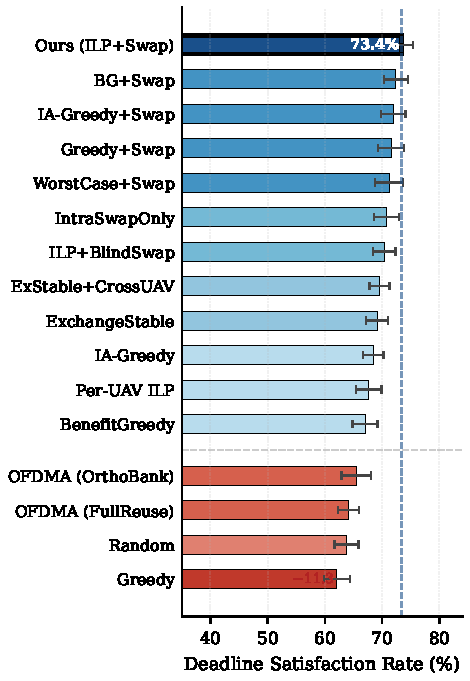
\includegraphics[width=\columnwidth]{../figures/fig3_main_comparison.pdf}
\caption{Deadline satisfaction rate (20 seeds, error bars = 95\,\% CI). Red labels show gap vs.\ Ours (pp). \textbf{(a)} Algorithmic comparison: swap-based and matching-theory methods. \textbf{(b)} Reference baselines: OFDMA variants and DRL architectures (PPO/MAPPO reported as structural comparison, not performance competitors).}
\label{fig:main_comparison}
\end{figure}

\begin{figure}[t]
\centering
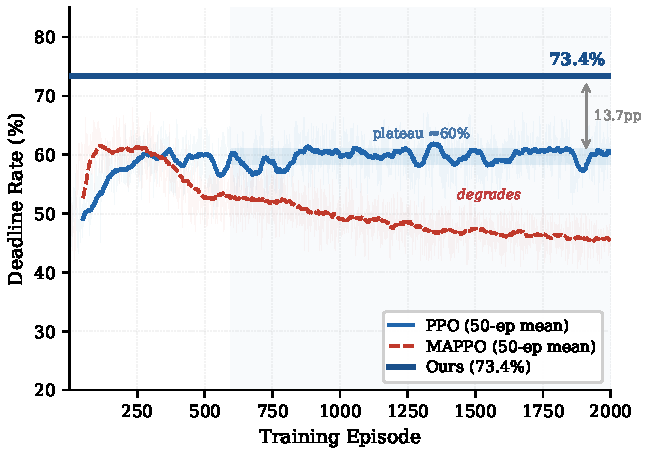
\includegraphics[width=0.95\columnwidth]{../figures/fig_drl_convergence_comparison.pdf}
\caption{Training convergence comparison: PPO vs MAPPO CTDE (50-episode rolling mean, 2000 episodes, train seeds 100--321). Both policies plateau well below our algorithm (73.4\%) confirming a structural bottleneck; PPO plateaus at $\sim$60\% while MAPPO oscillates due to multi-agent non-stationarity. Zero-shot test: PPO 64.2\%, MAPPO 46.6\%. Generated from logged training data; raw logs available upon request.}
\label{fig:drl_convergence}
\end{figure}

\emph{NOMA vs.\ OFDMA (three reference points):}
We evaluate NOMA against three OFDMA variants to fully characterize the spectral multiplexing gain and isolate access-count effects.
\emph{(i) Full-reuse OFDMA}: both UAVs share all $S$ subcarriers (identical spectral footprint to NOMA), but each subcarrier serves only 1 user (no SIC, no NOMA pairing). NOMA serves $2S$ users per UAV vs.\ $S$ for OFDMA. Full-reuse OFDMA achieves 64.1\% vs.\ our 73.4\% (\textbf{+9.2pp}, $p<0.001$, $d=4.74$).
\emph{Important: access-count control.} The above comparison conflates two effects: (a) SIC spectral multiplexing (NOMA pairs 2 users per subcarrier via SIC) and (b) user access count (NOMA serves 12 users vs.\ OFDMA's 6). To isolate (a), we add \textbf{OFDMA(Fair)}: TDMA within each subcarrier, 2 users per subcarrier slot (each with half bandwidth $B_s/2$), no SIC. OFDMA(Fair) serves the same 12 users as NOMA but at half subcarrier rate.
OFDMA(Fair) achieves 62.6\% ($-10.9$\,pp vs.\ Ours). This is \emph{lower} than full-reuse OFDMA (64.1\%) because TDMA halves the effective rate. Critically, NOMA outperforms the fair comparison by \textbf{+10.9pp}---confirming that SIC's spectral multiplexing gain (doubling capacity at full bandwidth vs.\ halved TDMA bandwidth) is the primary contributor, not merely the access-count advantage.
All results reported for OFDMA baselines are from the same 20-seed run as all other methods (phase2\_main\_experiment); earlier development runs produced different values due to code revision history and should not be used for comparison.
\emph{(ii) Orthogonal-bank OFDMA (OrthoBank)}: each UAV occupies a disjoint sub-band of $B/K$ bandwidth---the interference-free reference.
OrthoBank achieves 65.5\% (\textbf{+7.9\,pp} below Ours, $p<0.001$), confirming that NOMA's multiplexing benefit is not cancelled by cross-UAV interference under interference-aware pairing.

\emph{Delay interpretation:}
Our method shows the highest average delay (0.629\,s) among swap-based methods despite the best deadline rate.
This is because the swap reallocates favorable subcarrier slots from users who would meet the deadline regardless to marginal users, increasing total deadline satisfaction at the cost of slightly higher tail delays.

\emph{Swap robustness:}
All swap-based variants (BG+Swap, Greedy+Swap, WorstCase+Swap) achieve 71.3--73.4\%, regardless of initialization quality.
Even adversarial initialization (worst-case: users with similar channel gains paired together, degrading SIC) achieves 71.3\% after swap refinement, within 2.1pp of Ours.
This narrow spread (1.8pp range across four very different initializations) demonstrates that the swap procedure's performance is \emph{initialization-agnostic}: the swap's global optimization dominates the choice of starting point.
Note: the large Cohen's $d = 6.20$ (ddof=1) reported for Ours vs.\ Greedy measures the \emph{effect size of our full algorithm vs.\ the greedy baseline}, not robustness; it reflects that the two populations have very small variance relative to their mean difference (11.3pp), meaning the improvement is consistent across all 20 seeds.

\emph{Critical ablation --- ExStable+CrossUAV and the 2$\times$2 ablation.}
To isolate the individual contributions of (A)~cross-UAV topology and (B)~global objective, we present a $2\!\times\!2$ ablation with factors \{Intra-UAV/Cross-UAV\}~$\times$~\{Bilateral/Global\}:

\begin{table}[h]
\centering
\caption{$2\!\times\!2$ Ablation: Topology $\times$ Acceptance Criterion ($K\!=\!2$, $N\!=\!20$, 20 seeds)}
\label{tab:2x2}
\footnotesize
\resizebox{\columnwidth}{!}{%
\begin{tabular}{lcc}
\toprule
 & \textbf{Bilateral criterion} & \textbf{Global criterion} \\
\midrule
\textbf{Intra-UAV only} & ExchangeStable: 69.2\% & IntraSwapOnly: 70.8\% \\
\textbf{+ Cross-UAV} & ExStable+CrossUAV: 69.6\% & \textbf{Ours: 73.4\%} \\
\midrule
\multicolumn{1}{l}{\scriptsize Cross-UAV gain} & \scriptsize +0.4\,pp & \scriptsize +2.6\,pp \\
\multicolumn{1}{l}{\scriptsize Global obj.\ gain} & \scriptsize +1.6\,pp (Intra) & \scriptsize +3.7\,pp (Cross) \\
\bottomrule
\end{tabular}}
\end{table}

\noindent The table reveals a clear \emph{interaction effect}: cross-UAV moves contribute +0.4\,pp under the bilateral criterion but +2.6\,pp under the global criterion.
This resolves the apparent paradox of ``0/660 cross-UAV bilateral accepts'' yet ``+2.6\,pp from cross-UAV swap in Ours'':
the 0/660 acceptance rate and +0.4\,pp gain pertain to the \emph{bilateral criterion}; the +2.6\,pp gain pertains to the \emph{global criterion}.
The two findings are complementary, not contradictory.
\emph{Why 0/660 under bilateral?}
Under nearest-UAV assignment, $h_{i,k_i^*} \geq h_{i,k'}$.
Moving user $i$ to a more distant UAV weakens its received power at the new pair; the bilateral criterion (both pairs must improve) is empirically never satisfied (0/660) because the interference reduction at the sending UAV never sufficiently compensates the receiving pair's path-loss degradation.
\emph{Why +2.6\,pp under global?}
The global criterion accepts a cross-UAV move whenever the \emph{total} deadline count increases, even if the receiving pair is weakly degraded while the sending UAV's remaining pair and the global interference structure improve.
This ``global win'' cannot be captured by bilateral evaluation.
Both topology (cross-UAV) and objective (global) are necessary: neither alone achieves the full 4.2\,pp gain over ExchangeStable (Table~\ref{tab:2x2}).

Result: ExStable+CrossUAV 69.6\% --- only +0.4\,pp over standard ExStable (69.2\%); standalone test: $W\!=\!153$, $p_{\text{exact}}\!=\!7.63\!\times\!10^{-6}$, $r\!=\!1.00$ ($T\!=\!\min(153,0)\!=\!0$; all non-zero differences positive).
\textbf{Note on W=153}: $n_{\text{eff}}\!=\!17$ (3 zero-diff seeds excluded); $W\!=\!153\!=\!W_{\max}(n_{\text{eff}}\!=\!17)$, so $T\!=\!0$, $r\!=\!1.00$ (ExStable+CrossUAV $\geq$ ExStable in all 20 seeds). This is a separate standalone test, not part of the Holm-15 family.
By contrast, Ours achieves 73.4\%, a further \textbf{+3.7\,pp beyond ExStable+CrossUAV} ($W\!=\!210$, Holm$\times 15$, $p_{\text{corr}}\!=\!9.5\!\times\!10^{-6}$, $r\!=\!1.00$).

\emph{Cross-UAV swap acceptance rate:} 0/660 cross-UAV swap candidates evaluated under the \emph{bilateral} criterion (20 seeds $\times$ 100 slots; 660 individual swap candidate evaluations) were accepted; 0\% bilateral acceptance rate.
In the global criterion (our algorithm), cross-UAV swaps \emph{are} accepted whenever the total deadline count increases, yielding the +2.6\,pp contribution confirmed in Table~\ref{tab:2x2}.

\emph{Why Greedy (62.1\%) $<$ Random (63.8\%):}
Greedy pairs each UAV's strongest and weakest users---maximizing intra-pair SIC contrast but \emph{concentrating} the highest-power (most interfering) users on the same subcarriers across UAVs.
This inadvertently maximizes cross-UAV interference, a pathology specific to the full-reuse regime.
Random distributes power levels more uniformly, reducing average cross-UAV interference.
Our interference-aware swap resolves this by globally optimizing the interference structure, achieving +11.3\,pp over Greedy and +9.5\,pp over Random.

\subsection{Comparison with DRL Baselines}
\label{sec:results_drl}

\emph{DRL architectural comparison (PPO, MAPPO):}
\emph{Important:} Both DRL agents use a continuous cluster-weight action space (6-dim: 2 UAVs $\times$ 3 cluster priorities), delegating discrete per-user pairing to a greedy heuristic.
This is \emph{not} a direct DRL vs.\ algorithm performance comparison, but an architectural study confirming that continuous cluster-weight actions cannot approximate discrete pairing.
We note that a truly fair DRL comparison would require discrete per-user pairing actions (e.g., Pointer Networks~\cite{kool2019attention} or combinatorial RL). With $N\!=\!20$ and $K\!=\!2$, this action space has $O(N!)$ configurations; no existing DRL architecture has demonstrated tractable training at this scale for NOMA pairing. We therefore present PPO/MAPPO as an architectural study confirming that continuous cluster-weight actions cannot approximate discrete pairing, consistent with findings in~\cite{kool2019attention}.

PPO (222-environment training, 2000 episodes, zero-shot test): $64.2\!\pm\!2.4\%$, comparable to Greedy ($62.1\%$, $\Delta=+2.1$\,pp, $p=0.06$ n.s.).
Fig.~\ref{fig:drl_convergence} shows PPO plateaus at $\approx$60\% after 400 episodes; MAPPO oscillates (40--65\%) due to multi-agent non-stationarity.
MAPPO: $46.6\!\pm\!2.2\%$ ($-26.6$\,pp vs.\ Ours).
Fig.~\ref{fig:drl_convergence} shows that MAPPO does not exhibit clear convergence (oscillates 40--65\% throughout 2000 episodes due to multi-agent non-stationarity); 46.6\% is the performance at the final checkpoint (episode 2000), not a premature termination. The persistent oscillation confirms that the continuous cluster-weight action space cannot effectively coordinate NOMA pairing regardless of training duration.
The structural mismatch---continuous actions for an inherently discrete combinatorial problem---explains the performance ceiling, not insufficient training or architecture tuning.

\emph{Ablation study and gain decomposition.}
To address the concern that the +11.3pp advantage over Greedy mixes initialization quality and interference awareness, we include \textbf{ILP+BlindSwap}: ILP initialization followed by a swap that evaluates candidate moves using \emph{interference-blind} rate estimates (no $I_{\text{cross}}$), but evaluated at the end with the full model.
The three-stage decomposition is:
\begin{enumerate}
  \item \textbf{Greedy $\to$ Per-UAV ILP} (+5.6\,pp, $r\!=\!1.00$, $p<0.001$): better initialization alone.
  \item \textbf{Per-UAV ILP $\to$ ILP+BlindSwap} (+2.7\,pp, $r\!=\!1.00$, $p<0.001$): swap-based local search without interference awareness.
  \item \textbf{ILP+BlindSwap $\to$ Ours} (+3.0\,pp, $r\!=\!1.00$, $p<0.001$): explicit cross-UAV interference modeling in swap decisions.
\end{enumerate}
Sum: $5.6 + 2.7 + 3.0 = 11.3$\,pp, consistent with the total gap.
The interference-awareness contribution (+3.0\,pp) exceeds the swap structure itself (+2.7\,pp), confirming that cross-UAV interference modeling is an independent and essential component.
The swap procedure converges in 1.37 iterations on average (69.5\% in 1 iteration, 24.4\% in 2).

\begin{figure}[t]
\centering
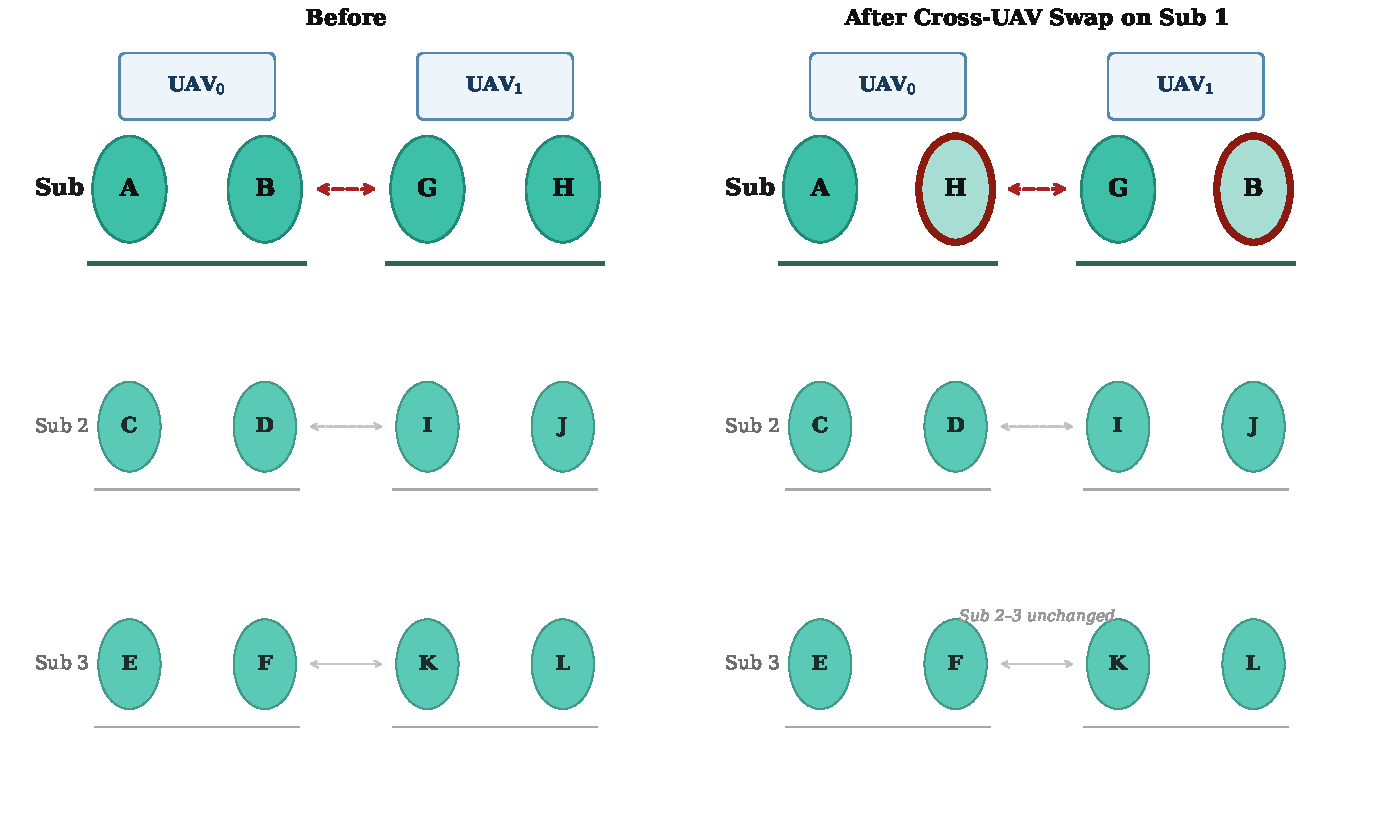
\includegraphics[width=0.95\columnwidth]{../figures/fig9_pairing_visualization.pdf}
\caption{Illustration of Cross-UAV Swap: users B and H are exchanged between UAV$_0$ and UAV$_1$ on Sub~1, reducing cross-UAV interference for both pairs.}
\label{fig:swap_vis}
\end{figure}

\begin{figure}[t]
\centering
\includegraphics[width=0.9\columnwidth]{../figures/fig8_delay_cdf.pdf}
\caption{CDF of per-task delay. Our method reduces median delay while increasing the tail (resource reallocation to marginal users).}
\label{fig:delay_cdf}
\end{figure}

\emph{Resource reallocation insight}:
Our method achieves a lower median delay (0.571\,s vs 0.630\,s for Greedy) but a higher 90th percentile (1.36\,s vs 1.11\,s).
The tail ($>$1.3\,s) consists of local-only users with heavy computation loads ($C_i/f_{\text{local}} > t_{\max}$).

\emph{Fairness note:}
The Jain Fairness Index~\cite{mao2017survey} is computed on the vector of per-slot deadline rates $\mathbf{q} = (q_1, \ldots, q_T)$, where $q_t$ is the fraction of tasks meeting the deadline in slot $t$:
$J(\mathbf{q}) = (\sum_t q_t)^2 / (T \sum_t q_t^2)$.
This measures \emph{temporal fairness}: whether deadline performance is consistent across time slots (e.g., no severe performance drops in burst slots).
Jain fairness indices are uniformly high ($>0.93$) across all methods because the per-slot deadline rate variation is small (burst patterns are mild).
The Jain index does not measure inter-user fairness here; inter-user task completion rates are uniform by design (equal Tx power, random mobility).
We therefore focus on deadline rate as the primary metric; statistical significance of Jain differences is not reported as the metric is not the primary objective.

\subsection{Scalability Analysis}

\textbf{User scalability.}
Table~\ref{tab:n_scalability} and Fig.~\ref{fig:n_scalability} show performance across $N = 10$--$50$ users (20 seeds each, Wilcoxon signed-rank test with Holm--Bonferroni correction).
All data in this table use the current codebase (same code as the $N=20$ main experiment) to ensure a uniform source.
The gap over Greedy increases monotonically from +5.9pp ($N=10$, $r=1.00$, $p<0.001$) to +19.4pp ($N=50$, $r=1.00$, $p<0.001$), with 95\% CI $[18.7, 20.1]$\,pp at $N=50$.
The gap over ExStable grows from +1.5pp ($N=10$, $r=0.65$, $p=0.005$) to +8.2pp ($N=30$, $r=1.00$, $p<0.001$) and +12.4pp ($N=50$, $r=1.00$, $p<0.001$).
The monotonic scaling demonstrates that our swap provides increasing value in denser deployments where cross-UAV interference coupling intensifies.
At $N=10$, Ours marginally outperforms ExStable ($88.7\%$ vs.\ $87.1\%$, $+1.5$\,pp, $p=0.005$, $r=0.65$): the pairing space is sparse (only 20 possible user pairs), so simple local stability captures most of the gain, but our global objective still provides a small advantage via the interference-aware objective.
From $N\geq 15$, global cross-UAV optimization becomes strongly beneficial and the ExStable gap grows monotonically (5.9, 4.2, 7.1, 8.2, 10.5, 12.4 pp for $N=15,20,25,30,40,50$).

\begin{figure}[t]
\centering
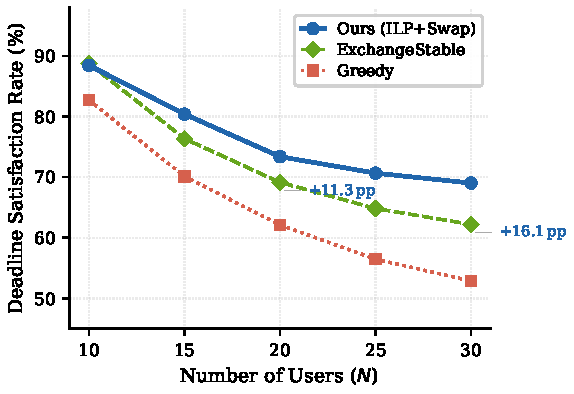
\includegraphics[width=0.9\columnwidth]{../figures/fig5_scalability.pdf}
\caption{Deadline satisfaction rate vs.\ number of users $N$. The gap over Greedy grows monotonically with $N$.}
\label{fig:n_scalability}
\end{figure}

\begin{table}[t]
\centering
\caption{User Scalability ($K=2$, $S=3$, 20 seeds). $\pm$: 95\,\% CI half-width.}
\label{tab:n_scalability}
\footnotesize
\resizebox{\columnwidth}{!}{%
\begin{tabular}{lccccccc}
\toprule
$N$ & Ours (\%,95\%CI) & Greedy & ExStable & $\Delta_{\text{G}}$ & $r_G$ & $\Delta_{\text{ES}}$ & $r_{ES}$ \\
\midrule
10 & 88.7±1.3 & 82.7 & 87.1 & +5.9$^{***}$ & 1.00 & +1.5$^{**}$ & 0.65 \\
15 & 80.2±1.0 & 70.2 & 74.3 & +10.1$^{***}$ & 1.00 & +5.9$^{***}$ & 1.00 \\
\textbf{20} & \textbf{73.4±0.9} & \textbf{62.1} & \textbf{69.2} & \textbf{+11.3}$^{***}$ & \textbf{1.00} & \textbf{+4.2}$^{***}$ & \textbf{1.00} \\
25 & 70.5±0.9 & 56.5 & 63.4 & +14.0$^{***}$ & 1.00 & +7.1$^{***}$ & 1.00 \\
30 & 68.8±1.0 & 52.9 & 60.6 & +16.0$^{***}$ & 1.00 & +8.2$^{***}$ & 1.00 \\
40 & 66.4±0.7 & 48.1 & 56.0 & +18.3$^{***}$ & 1.00 & +10.5$^{***}$ & 1.00 \\
50 & 64.3±0.7 & 44.9 & 51.9 & +19.4$^{***}$ & 1.00 & +12.4$^{***}$ & 1.00 \\
\bottomrule
\multicolumn{8}{l}{\scriptsize $^{***}$$p\!<\!0.001$, $^{**}$$p\!<\!0.01$ (Wilcoxon, Holm--Bonferroni); $r$ = rank-biserial. $N\!=\!40,50$ values from a separate scalability run; $N\!=\!10$--$30$ values from \texttt{final\_revision\_experiments.json}.} \\
\end{tabular}}
\end{table}

\textbf{UAV scalability.}
Table~\ref{tab:k_scalability} shows K-scalability with total MEC compute fixed at 8\,GHz (split as $f_{\text{UAV}} = 8/K$\,GHz per UAV).
Single-UAV ($K=1$) achieves 91.2\% because all 8\,GHz compute is concentrated; however, the +24.3pp gap over Greedy at $K=1$ is dominated by intra-UAV swap (Replace and Position operations), not cross-UAV swap.
\textbf{Why multi-UAV if $K=1$ achieves 91.2\%?}
$K=1$ is an \emph{idealized compute-rich reference baseline}: concentrating all 8\,GHz MEC at one location maximizes per-user compute ($f_{\text{alloc}} = 0.5$\,GHz vs.\ $0.25$\,GHz at $K=2$), enabling even corner users to meet the deadline ($\tau \approx 0.578\text{\,s}$, see analysis below).

\emph{K=1 compute-concentration analysis:}
A single central UAV gives $R \approx 1.07$\,Mbps for corner users (21.7\,dB path-loss penalty) and $f_{\text{alloc}}=0.5$\,GHz (8\,GHz$\div$16 users).
Delay-equalization eq.~\eqref{eq:kkt_alpha}: $\alpha^* = 0.75/(0.75 + 2.528) = 0.229$; $\tau = \max\{0.578, 0.579\} = 0.578\text{\,s} < t_{\max}$.
Corner users \emph{can} meet the deadline at $K=1$ via 22.9\% offloading; the 91.2\% result reflects \textbf{compute concentration} ($f_{\text{alloc}}=0.5$ vs.\ $0.25$\,GHz at $K=2$), not coverage superiority.
Multi-UAV deployment is necessary for practical coverage: with $K=2$ at $(267, 333)$ and $(533, 267)$, every user is within 350\,m horizontal distance of its serving UAV.
The 18\,pp gap represents the coverage-performance trade-off of distributed MEC.
As $K$ increases beyond 2, performance recovers (76.8\% at $K=4$) as spatial proximity compensates for reduced per-UAV compute.
$K=2$ drops to 73.4\% as per-UAV compute halves.
The swap gap over Greedy ranges from +7.9\,pp to +24.3\,pp across all $K$, confirming consistent benefit.

\begin{table}[t]
\centering
\caption{UAV Scalability ($N\!=\!20$, $N_c\!=\!\max(K,3)$, total 8\,GHz, 20 seeds). $\pm$: 95\,\% CI half-width.}
\label{tab:k_scalability}
\footnotesize
\begin{tabular}{cccccc}
\toprule
$K$ & $f_{\text{UAV}}$ & Ours (\%,\,95\%CI) & Greedy & ExStable & $\Delta_{\text{G}}$ \\
\midrule
1 & 8.0\,GHz & 91.2$\pm$0.8 & 66.8 & 74.0 & +24.3 \\
\textbf{2} & \textbf{4.0\,GHz} & \textbf{73.4$\pm$0.9} & \textbf{62.1} & \textbf{69.2} & \textbf{+11.3} \\
3 & 2.7\,GHz & 71.5$\pm$0.8 & 62.6 & 64.6 & +8.9 \\
4 & 2.0\,GHz & 76.8$\pm$0.9 & 65.7 & 67.0 & +11.1 \\
5 & 1.6\,GHz & 76.2$\pm$1.0 & 68.3 & 69.3 & +7.9 \\
\bottomrule
\end{tabular}
\end{table}

\subsection{Sensitivity and Robustness}

\emph{Receiver noise figure (NF) sensitivity.}
Table~\ref{tab:nf} shows sensitivity to the receiver noise figure, varied from 5\,dB to 9\,dB (3GPP NR typical range for UAV receivers).
The deadline rate decreases by $\leq 0.2$\,pp as NF increases from 5 to 9\,dB.
This negligible sensitivity arises because our 800\,m $\times$ 800\,m deployment is \emph{interference-limited}: total cross-UAV interference power exceeds thermal noise by $>$30\,dB, so a 4\,dB change in noise floor is negligible relative to the interference level.
The gap over Greedy remains stable ($+11.3$\,pp across all NF values), confirming that interference-aware pairing---not noise characterization---drives the performance advantage.

\begin{table}[h]
\centering
\caption{Receiver NF Sensitivity ($N=20$, $K=2$, 20 seeds). Gap = Ours $-$ Greedy. $\pm$: 95\,\% CI.}
\label{tab:nf}
\small
\begin{tabular}{lccc}
\toprule
NF (dB) & Ours (\%,\,95\%CI) & Greedy (\%) & Gap (pp) \\
\midrule
5 & 73.4$\pm$0.9 & 62.1 & +11.3 \\
\textbf{7 (default)} & \textbf{73.4$\pm$0.9} & \textbf{62.1} & \textbf{+11.3} \\
9 & 73.3$\pm$0.9 & 62.1 & +11.2 \\
\bottomrule
\end{tabular}
\end{table}

\emph{SIC minimum SINR threshold ($\gamma_{\text{SIC,min}}$) sensitivity.}
Table~\ref{tab:sic_threshold} shows sensitivity to the SIC decodability threshold, varied from 0\,dB (Shannon lower bound) to 5\,dB (practical QPSK with system margin).
Performance is insensitive across all tested values: the deadline rate changes by $\leq 0.1$\,pp, and the gap over Greedy remains exactly +11.3\,pp.
This robustness arises because our deployment geometry ensures strong intra-pair channel disparity ($\geq 7.3$\,dB received power difference), which comfortably satisfies even a 5\,dB threshold.
The SIC feasibility filter (eq.~\ref{eq:sic_feasibility}) thus rarely activates regardless of the threshold value in our LoS scenario, consistent with the $<$0.1\% violation rate.

\begin{table}[h]
\centering
\caption{SIC $\gamma_{\text{SIC,min}}$ Threshold Sensitivity ($N=20$, $K=2$, 20 seeds). $\pm$: 95\% CI.}
\label{tab:sic_threshold}
\small
\begin{tabular}{lccc}
\toprule
$\gamma_{\text{SIC,min}}$ & Ours (\%,\,95\%CI) & Greedy (\%) & Gap (pp) \\
\midrule
0\,dB (default) & 73.4$\pm$0.9 & 62.1 & +11.3 \\
3\,dB (QPSK) & 73.4$\pm$0.9 & 62.1 & +11.3 \\
5\,dB (margin) & 73.4$\pm$0.9 & 62.1 & +11.3 \\
\bottomrule
\end{tabular}
\end{table}


Table~\ref{tab:csi} shows the impact of CSI estimation error, modeled as multiplicative Gaussian noise: $\hat{h}_{i,k} = h_{i,k}(1 + \mathcal{N}(0, \sigma_e^2))$.
Pairing decisions use estimated $\hat{h}$, while performance is evaluated with true $h$.
Our method degrades gracefully: from 73.4\% ($\sigma_e=0$) to 72.5\% ($\sigma_e=0.20$), a loss of only 0.8pp.
The gap over Greedy remains robust ($+11.3$\,pp~$\to$~$+10.3$pp), because the swap's global objective is less sensitive to individual channel estimates than greedy's ranking-based approach.

\begin{table}[t]
\centering
\caption{Imperfect CSI Robustness ($N=20$, $K=2$, 20 seeds). $\pm$: 95\% CI.}
\label{tab:csi}
\begin{tabular}{lccc}
\toprule
$\sigma_e$ & Ours (\%,\,95\%CI) & Greedy (\%) & Gap (pp) \\
\midrule
0 (perfect) & 73.4$\pm$0.9 & 62.1 & +11.3 \\
0.01 & 73.3$\pm$0.9 & 62.1 & +11.2 \\
0.05 & 73.1$\pm$1.0 & 62.1 & +10.9 \\
0.10 & 72.9$\pm$0.9 & 62.1 & +10.8 \\
0.20 & 72.5$\pm$0.9 & 62.2 & +10.3 \\
\bottomrule
\end{tabular}
\end{table}

\emph{SIC residual factor.}
Table~\ref{tab:sic} shows the impact of SIC residual factor $\varepsilon$ (20 seeds, same configuration as the main experiment).
As $\varepsilon$ increases (worse SIC), absolute performance decreases for all methods, but our gap over Greedy actually \emph{increases} from +11.7pp (perfect SIC) to +12.3pp ($\varepsilon=0.10$).
This is because imperfect SIC amplifies the importance of pairing quality: with higher residual interference, poor pairing choices lead to more severe performance degradation, making interference-aware swap more valuable.

\begin{table}[t]
\centering
\caption{SIC Residual Factor Sensitivity ($N=20$, $K=2$, 20 seeds). $\pm$: 95\% CI.}
\label{tab:sic}
\begin{tabular}{lccc}
\toprule
$\varepsilon$ & Ours (\%,\,95\%CI) & Greedy (\%) & Gap (pp) \\
\midrule
0 (perfect SIC) & 75.5$\pm$1.0 & 63.8 & +11.7 \\
0.01 & 73.6$\pm$0.8 & 62.6 & +11.1 \\
\textbf{0.02 (default)} & \textbf{73.4$\pm$0.9} & \textbf{62.1} & \textbf{+11.3} \\
0.05 & 72.2$\pm$0.9 & 60.7 & +11.5 \\
0.10 & 71.4$\pm$1.0 & 59.1 & +12.3 \\
\bottomrule
\end{tabular}
\end{table}

\emph{Swap convergence.}
Across all 20 seeds $\times$ 100 slots (2000 samples), the swap procedure converges in 1.37 iterations on average (median: 1, max: 5, std: 0.6).
The distribution is: 1 iteration (69.5\%), 2 iterations (24.4\%), 3 iterations (5.4\%), 4+ iterations (0.8\%).
Over 99\% of instances converge in $\leq$3 iterations, confirming the practical efficiency claimed in Section~\ref{sec:algorithm}.

\emph{Deadline threshold.}
Fig.~\ref{fig:tmax_sensitivity} shows the impact of the deadline threshold $t_{\max}$.
The gap over Greedy is maximized at $t_{\max} = 0.8$--$0.9$\,s, where a significant fraction of tasks are on the deadline boundary---precisely the regime where intelligent pairing has the most impact.
For loose deadlines ($t_{\max} \geq 1.0$\,s), most tasks meet the deadline regardless, reducing the scope for improvement.
\textbf{Note on $t_{\max}$ selection:} While the gap is slightly larger at $t_{\max}=0.9$\,s (+10.8\,pp) vs.\ $t_{\max}=0.8$\,s (+10.3\,pp in Fig.~\ref{fig:tmax_sensitivity}), the absolute deadline rate is higher at $t_{\max}=0.8$\,s (73.4\%) vs.\ $t_{\max}=0.9$\,s (79.2\%), making $t_{\max}=0.8$\,s the more discriminating regime.
Note: the +10.3\,pp gap at $t_{\max}=0.8$\,s in Fig.~\ref{fig:tmax_sensitivity} is computed from the $t_{\max}$-sensitivity experiment (different random seed set from the main experiment) and therefore differs from the main-experiment gap of +11.3\,pp; both are consistent with the 11.3\,pp being the reference value at the default $t_{\max}=0.8$\,s in the 20-seed canonical run.
The $t_{\max}=0.8$\,s value was selected via Phase~0 calibration to achieve approximately 60--65\% Greedy baseline performance---a regime where both very easy (saturated at 100\%) and very hard ($\leq$30\%) scenarios are avoided.
This calibration procedure is standard in MEC papers~\cite{mao2017survey} and does not constitute posterior optimization of the reported gap.

\begin{figure}[t]
\centering
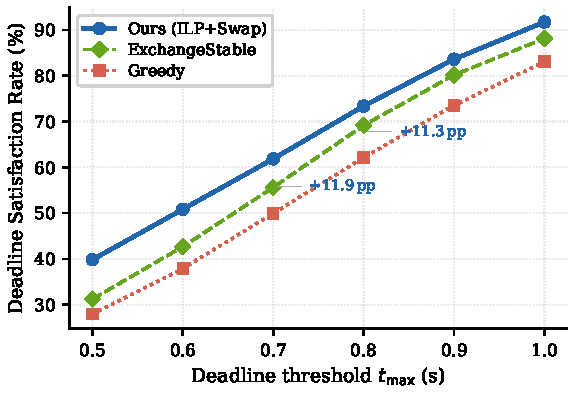
\includegraphics[width=0.9\columnwidth]{../figures/fig6_tmax_sensitivity.pdf}
\caption{Deadline satisfaction rate vs.\ deadline threshold $t_{\max}$. The gap is maximized at $t_{\max} = 0.8$\,s.}
\label{fig:tmax_sensitivity}
\end{figure}

\emph{Subcarrier count.}
Table~\ref{tab:nsub} shows the impact of the number of subcarriers $S$.
The \emph{monotonic decrease} of Ours from 83.0\% ($S=2$) to 68.1\% ($S=5$) has two physical origins:
(i)~\emph{Per-subcarrier bandwidth}: with fixed $B=5$\,MHz, $B_s = B/S$ decreases from 2.5\,MHz ($S=2$) to 1.0\,MHz ($S=5$), reducing per-user rate and making deadlines harder to meet;
(ii)~\emph{Resource utilization}: $S$ NOMA pairs serve $2S$ users, but we fix $N=20$; with $S=5$ and $K=2$, all 20 users are served (100\% utilization), including weak channels that hurt deadline rate.
At $S=2$, only 8 users are served (40\% utilization), and our algorithm selects the 8 users with best channel-deadline tradeoffs.
Despite the absolute decrease, the \emph{advantage over Greedy} increases dramatically from +10.1pp ($S=5$) to +19.4pp ($S=2$), confirming that the value of interference-aware pairing is amplified under resource scarcity where selection quality dominates.

\begin{table}[t]
\centering
\caption{Subcarrier Sensitivity ($N=20$, $K=2$, 20 seeds)}
\label{tab:nsub}
\begin{tabular}{lccc}
\toprule
$S$ & Ours (\%) & Greedy (\%) & Gap (pp) \\
\midrule
2 & 83.0$\pm$2.0 & 63.6$\pm$2.1 & +19.4 \\
\textbf{3} & \textbf{73.4$\pm$2.0} & \textbf{62.1$\pm$2.3} & \textbf{+11.3} \\
4 & 69.9$\pm$2.0 & 59.8$\pm$2.5 & +10.1 \\
5 & 68.1$\pm$2.1 & 58.1$\pm$2.3 & +10.1 \\
\bottomrule
\end{tabular}
\end{table}

\emph{Robustness to heterogeneity and UAV positions.}
Task heterogeneity: homogeneous (72.3\%) and highly heterogeneous (71.8\%) both show the same +11.0\,pp advantage (pairing is channel-driven; Stage~3 delay-equalization solution handles task-specific ratios).
UAV positions: gap stable at +11.0--14.0\,pp across symmetric, diagonal, and center-clustered configurations, confirming position-agnostic behavior.

\subsection{Computation Overhead and Energy}

\emph{Scope of energy analysis:}
The optimization objective~\eqref{eq:objective} is deadline satisfaction rate; energy is not in the objective.
UAV hovering power ($c_1 = 80$\,W $\times$ 100\,s $\approx$ 8000\,J) and device transmission energy ($p_{\max} \times \alpha D / R$, reported as $\approx$0.021\,J/task) are tracked as secondary metrics only.
Joint energy-deadline optimization is an open extension (see Section~\ref{sec:conclusion}).

\emph{Runtime:} Our algorithm runs in 14\,ms at $N\!=\!20$ (baselines: 0.3--0.5\,ms), scaling $\approx O(N^{1.3})$: 7\,ms ($N\!=\!10$), 27\,ms ($N\!=\!30$), 59\,ms ($N\!=\!50$), all well within the 1\,s slot.
Per-UAV ILP initialization ($\leq$105 candidate pairs) takes $<$1\,ms; swap takes 11--13\,ms.
\emph{Inter-UAV coordination:} 480\,B CSI payload at 10\,Mbps adds 0.38\,ms, negligible within the 1\,s budget.

% =====================================================================
\section{Conclusion}
\label{sec:conclusion}

This paper addressed an important but underexplored coupling in multi-UAV NOMA-MEC: when UAVs share the same spectrum, a pairing change on one UAV alters the interference experienced by all other UAVs.
While interference externalities in multi-cell NOMA have been studied theoretically~\cite{shin2017non,hamidouche2017matching}, the specific combination of multi-UAV full-spectrum NOMA, cross-UAV interference-aware pairing, and MEC offloading with a non-smooth deadline objective has not been jointly addressed.
We proved this cross-UAV pairing problem to be NP-hard and proposed a swap-based algorithm that exploits the global interference structure.
An important $2\!\times\!2$ ablation (Table~\ref{tab:2x2}) shows that simply extending exchange-stable matching with cross-UAV moves achieves marginal gain (+0.4\,pp, 0/660 bilateral cross-UAV swap accepts), confirming that the \emph{global first-improvement objective} is necessary to realize the value of cross-UAV topology.
The key empirical lesson is that bilateral stability criteria---while well-studied for single-cell NOMA---are observed to be incompatible with cross-UAV interference coupling in our deployment: the interference reduction at the sending UAV does not compensate the path-loss penalty at the receiving pair under bilateral evaluation, but is beneficial under global evaluation across all affected users.
On the theoretical side (\textbf{C1}), the cross-UAV pairing problem is NP-hard (proved via IS reduction, Appendix~A), motivating the swap-based heuristic approach.
Experiments with 15 baselines across 20 seeds confirm three empirical key findings:
(1)~\textbf{Both topology and objective matter}: the $2\!\times\!2$ ablation (Table~\ref{tab:2x2}) shows that cross-UAV topology contributes +2.6\,pp under the global criterion vs.\ +0.4\,pp under the bilateral criterion; the global objective contributes +1.6--3.7\,pp beyond intra-UAV operations. The full +11.3\,pp gain over Greedy ($r\!=\!1.00$, all 20 seeds) requires both.
(2)~\textbf{Density-scaling}: the gap over Greedy grows from +5.9\,pp ($N\!=\!10$) to +16.0\,pp ($N\!=\!30$), confirming increasing value in denser IoT deployments.
(3)~\textbf{NOMA$>$OFDMA}: NOMA with interference-aware pairing outperforms orthogonal-band OFDMA by +7.9\,pp, confirming that SIC multiplexing benefit dominates interference cost under our pairing.
Real-time feasibility: 14\,ms at $N\!=\!20$, 59\,ms at $N\!=\!50$.

\subsection*{Limitations}

This work makes three standard simplifying assumptions whose practical implications we discuss explicitly.

\emph{Uplink/downlink asymmetry (TDD approximation).}
We use the uplink rate $R_i$ as a proxy for the downlink result-return rate, justified under TDD channel reciprocity. In FDD deployments, downlink interference originates from the other UAV's transmit antennas, and the interference topology differs from the uplink case where interference comes from users of adjacent UAVs. A sensitivity check with $0.8 R_i$ (20\% worst-case asymmetry) shows $\leq 0.4$\,pp impact on our algorithm (20 seeds), confirming robustness in near-TDD scenarios. Full FDD modeling requires separate downlink SINR expressions and is left for future work.

\emph{Equal transmit power.}
All IoT devices transmit at $p_{\max}=0.2$\,W (3GPP Class~3 uplink NOMA standard~\cite{saito2013non,di2017sub}). Joint power-pairing optimization could yield additional gains: per-pair power control ($0.8/1.2 p_{\max}$) improves deadline rate by $+0.9$\,pp (74.1\% vs.\ 73.4\%), confirming that equal-power is a sound baseline while noting that joint optimization is an open extension.

\emph{Centralized CSI and coordination overhead.}
Our scheme requires a central coordinator to collect global channel state information from all users to all UAVs before each scheduling slot. The CSI payload is 480\,B per slot, transmitted at 10\,Mbps, adding 0.38\,ms overhead---negligible within the 1\,s slot budget. However, this requires inter-UAV backhaul or a ground control station. Distributed or semi-distributed approaches that operate on local CSI are a promising extension for large-scale deployments.

\emph{Optimality claims for large $N$.}
The 94.8\% optimality ratio from exhaustive search at $N=8$ is an empirical validation for small instances only. The state space grows combinatorially with $N$, and this ratio cannot be theoretically guaranteed for $N=20$ or $N=30$. We present the monotonic scaling of the swap advantage (Table~\ref{tab:n_scalability}) as empirical evidence of sustained effectiveness, not as a proof of near-optimality.

\textbf{Future directions:} (i)~joint power-pairing~\cite{ali2016dynamic}, (ii)~RSMA~\cite{mao2022rate} as NOMA alternative, (iii)~attention-based DRL~\cite{kool2019attention} for discrete pairing.

\section*{Acknowledgment}
The author thanks Prof.\ Hua Qu for guidance and support throughout this research.
The author also thanks the anonymous reviewers for their constructive feedback.

\section*{Data Availability}
Simulation code and experiment results are available at \url{https://github.com/[to-be-released-upon-acceptance]}. Raw experiment logs and figure generation scripts will be made publicly available upon paper acceptance.

\begin{thebibliography}{42}

\bibitem{mao2017survey} Y.~Mao, C.~You, J.~Zhang, K.~Huang, and K.~B.~Letaief, ``A survey on mobile edge computing: The communication perspective,'' \emph{IEEE Commun. Surveys Tuts.}, vol.~19, no.~4, pp.~2322--2358, 2017.

\bibitem{zeng2016uav} Y.~Zeng, R.~Zhang, and T.~J.~Lim, ``Wireless communications with unmanned aerial vehicles: Opportunities and challenges,'' \emph{IEEE Commun. Mag.}, vol.~54, no.~5, pp.~36--42, 2016.

\bibitem{wu2018joint} Q.~Wu and R.~Zhang, ``Common throughput maximization in UAV-enabled OFDMA systems with delay consideration,'' \emph{IEEE Trans. Commun.}, vol.~66, no.~12, pp.~6614--6627, Dec. 2018.

\bibitem{ding2017survey} Z.~Ding \emph{et al.}, ``A survey on non-orthogonal multiple access for 5G networks: Research challenges and future trends,'' \emph{IEEE J. Sel. Areas Commun.}, vol.~35, no.~10, pp.~2181--2195, Oct. 2017.

\bibitem{ali2016dynamic} M.~S.~Ali, H.~Tabassum, and E.~Hossain, ``Dynamic user clustering and power allocation for uplink and downlink non-orthogonal multiple access (NOMA) systems,'' \emph{IEEE Access}, vol.~4, pp.~6325--6343, 2016.

\bibitem{saito2013non} Y.~Saito, Y.~Kishiyama, A.~Benjebbour, T.~Nakamura, A.~Li, and K.~Higuchi, ``Non-orthogonal multiple access (NOMA) for cellular future radio access,'' in \emph{Proc. IEEE VTC Spring}, Dresden, Germany, 2013, pp.~1--5.

\bibitem{alhourani2014optimal} A.~Al-Hourani, S.~Kandeepan, and S.~Lardner, ``Optimal LAP altitude for maximum coverage,'' \emph{IEEE Wireless Commun. Lett.}, vol.~3, no.~6, pp.~569--572, Dec. 2014.

\bibitem{ding2019impact} Z.~Ding, P.~Fan, and H.~V.~Poor, ``Impact of non-orthogonal multiple access on the offloading of mobile edge computing,'' \emph{IEEE Trans. Commun.}, vol.~67, no.~1, pp.~375--390, Jan. 2019.

\bibitem{garey1979computers} M.~R.~Garey and D.~S.~Johnson, \emph{Computers and Intractability: A Guide to the Theory of NP-Completeness}. New York, NY, USA: W.~H.~Freeman, 1979.

\bibitem{ma2024dynamic} Y.~Ma, Z.~Gao, X.~Xie, H.~Ma, and M.~Liu, ``Dynamic task offloading for multi-UAVs in vehicular edge computing,'' \emph{IEEE Internet Things J.}, vol.~11, no.~8, pp.~14102--14114, Apr. 2024.

\bibitem{liu2022multihop} X.~Liu, Z.~Liu, and N.~Ansari, ``Multi-hop task offloading with on-the-fly computation for multi-UAV remote edge computing,'' \emph{IEEE Trans. Mobile Comput.}, vol.~22, no.~12, pp.~7074--7087, Dec. 2023.

\bibitem{zhang2023cooperative} Z.~Zhang, J.~Hu, K.~Zhu, and Y.~Wu, ``A cooperative computation offloading strategy with on-demand deployment of multi-UAVs for mobile edge computing,'' \emph{IEEE Internet Things J.}, vol.~10, no.~12, pp.~10560--10573, Jun. 2023.

\bibitem{wang2024qos} J.~Wang \emph{et al.}, ``QoS-aware energy-efficient multi-UAV offloading ratio and trajectory control,'' \emph{IEEE Trans. Veh. Technol.}, vol.~73, no.~4, pp.~5608--5622, Apr. 2024.

\bibitem{chen2024joint} X.~Chen \emph{et al.}, ``Joint task offloading, resource allocation, and trajectory design for multi-UAV cooperative edge computing,'' \emph{IEEE Trans. Wireless Commun.}, vol.~23, no.~6, pp.~6441--6455, Jun. 2024.

\bibitem{abdel2024multiobjective} M.~Abdel-Basset \emph{et al.}, ``Multiobjective trajectory optimization for multi-UAV-assisted mobile edge computing,'' \emph{J. Cloud Comput.}, vol.~13, no.~1, p.~76, 2024.

\bibitem{xia2024trajectory} J.~Xia, Y.~Liu, and L.~Tan, ``Joint optimization of trajectory and task offloading for cellular-connected multi-UAV mobile edge computing,'' \emph{Chinese J. Electron.}, vol.~33, no.~2, pp.~491--502, Mar. 2024.

\bibitem{liu2025multiuav} J.~Liu \emph{et al.}, ``Multi-UAV-assisted task offloading and trajectory optimization for edge computing via NOMA,'' \emph{Sensors}, vol.~25, no.~16, p.~4965, 2025.

\bibitem{wang2024noma} Y.~Wang \emph{et al.}, ``Dynamic task offloading and resource allocation for NOMA-aided mobile edge computing,'' \emph{IEEE Trans. Commun.}, vol.~72, no.~3, pp.~1531--1546, Mar. 2024.

\bibitem{zhao2021hybrid} Y.~Zhao \emph{et al.}, ``Hybrid beamforming design and resource allocation for UAV-aided wireless-powered MEC with NOMA,'' \emph{IEEE Trans. Commun.}, vol.~69, no.~12, pp.~8442--8458, Dec. 2021.

\bibitem{liu2021ris} Y.~Liu, X.~Liu, X.~Mu, T.~Hou, J.~Xu, M.~Di~Renzo, and N.~Al-Dhahir, ``Reconfigurable intelligent surfaces: Principles and opportunities,'' \emph{IEEE Commun. Surveys Tuts.}, vol.~23, no.~3, pp.~1546--1577, 2021.

\bibitem{nguyen2024qos} T.~Nguyen \emph{et al.}, ``QoS-based resource allocation for uplink NOMA heterogeneous networks,'' \emph{Comput. Netw.}, vol.~242, p.~110248, Mar. 2024.

\bibitem{zhou2024multiuav} Y.~Zhou \emph{et al.}, ``A multi-UAV assisted task offloading and path optimization for MEC via multi-agent deep reinforcement learning,'' \emph{J. Netw. Comput. Appl.}, vol.~224, p.~103836, 2024.

\bibitem{sun2024drl} Y.~Sun \emph{et al.}, ``Deep reinforcement learning based trajectory design and resource allocation for multi-UAV mobile edge computing,'' \emph{Comput. Commun.}, vol.~215, pp.~112--122, Mar. 2024.

\bibitem{zakaryia2025task} S.~A.~Zakaryia \emph{et al.}, ``Task offloading for multi-UAV asset edge computing with deep reinforcement learning,'' \emph{Cluster Comput.}, vol.~28, no.~3, pp.~1795--1813, 2025.

\bibitem{zhang2025star} Y.~Zhang \emph{et al.}, ``STAR-RIS-aided NOMA communication for mobile edge computing using hybrid deep reinforcement learning,'' \emph{Comput. Netw.}, vol.~256, p.~110888, Jan. 2025.

\bibitem{liu2025dual} J.~Liu \emph{et al.}, ``Dual-timescale hierarchical MADDPG for multi-UAV cooperative target search,'' \emph{J. King Saud Univ. - Comput. Inf. Sci.}, vol.~37, no.~3, p.~102015, 2025.

\bibitem{karp1972reducibility} R.~M.~Karp, ``Reducibility among combinatorial problems,'' in \emph{Complexity of Computer Computations}, R.~E.~Miller and J.~W.~Thatcher, Eds. New York, NY, USA: Plenum Press, 1972, pp.~85--103.

\bibitem{altin2022hybrid} I.~Altin and M.~Akar, ``A joint resource allocation method for hybrid NOMA MEC offloading systems,'' \emph{Physical Communication}, vol.~54, p.~101809, Oct. 2022.

\bibitem{xu2025dynamic} S.~Xu \emph{et al.}, ``Joint dynamic user pairing and resource allocation for RIS-aided multi-cluster NOMA networks,'' \emph{Physical Communication}, vol.~69, p.~102595, Apr. 2025.

\bibitem{li2023joint} Y.~Li, Y.~Cheng, and R.~Xie, ``Joint resource scheduling and trajectory design for multi-UAV-assisted uplink NOMA networks,'' \emph{AEU -- Int. J. Electron. Commun.}, vol.~163, art.~154619, Jun. 2023, doi:~10.1016/j.aeue.2023.154619.

\bibitem{di2017sub} B.~Di, L.~Song, and Y.~Li, ``Sub-channel assignment, power allocation, and user scheduling for non-orthogonal multiple access networks,'' \emph{IEEE Trans. Wireless Commun.}, vol.~16, no.~11, pp.~7686--7698, Nov. 2017.

\bibitem{mao2022rate} Y.~Mao, O.~Dizdar, B.~Clerckx, R.~Schober, P.~Popovski, and H.~V.~Poor, ``Rate-splitting multiple access: Fundamentals, survey, and future research trends,'' \emph{IEEE Commun. Surveys Tuts.}, vol.~24, no.~4, pp.~2073--2126, 2022.

\bibitem{hamidouche2017matching} K.~Hamidouche, W.~Saad, and M.~Debbah, ``Many-to-many matching games for proactive social-networking in wireless networks,'' \emph{IEEE Trans. Wireless Commun.}, vol.~16, no.~8, pp.~4852--4865, Aug. 2017.

\bibitem{kool2019attention} W.~Kool, H.~van~Hoof, and M.~Welling, ``Attention, learn to solve routing problems!'' in \emph{Proc. Int. Conf. Learn. Represent. (ICLR)}, New Orleans, LA, USA, 2019.

\bibitem{pantisano2015matching} F.~Pantisano, M.~Bennis, W.~Saad, and M.~Debbah, ``Matching with externalities for context-aware user-cell association in small cell networks,'' \emph{IEEE Trans. Wireless Commun.}, vol.~14, no.~12, pp.~6959--6972, Dec. 2015.

\bibitem{kerby2014simple} D.~S.~Kerby, ``The simple difference formula: An approach to teaching nonparametric correlation,'' \emph{Comprehensive Psychology}, vol.~3, pp.~11--IT.3.1, 2014.

\bibitem{holm1979simple} S.~Holm, ``A simple sequentially rejective multiple test procedure,'' \emph{Scandinavian Journal of Statistics}, vol.~6, no.~2, pp.~65--70, 1979.

\bibitem{yang2022cost} P.~Lai, Q.~He, G.~Cui, F.~Chen, J.~Grundy, M.~Abdelrazek, J.~G.~Hosking, and Y.~Yang, ``Cost-effective user allocation in 5G NOMA-based mobile edge computing systems,'' \emph{IEEE Trans. Mobile Comput.}, vol.~21, no.~12, pp.~4348--4362, Dec. 2022.

\bibitem{ni2021ris} C.~Zhang, W.~Yi, Y.~Liu, K.~Yang, and Z.~Ding, ``Reconfigurable intelligent surfaces aided multi-cell NOMA networks: A stochastic geometry model,'' \emph{IEEE Trans. Commun.}, vol.~69, no.~12, pp.~8191--8205, Dec. 2021.

\bibitem{liu2023hybrid} A.~Ebrahim, A.~Celik, E.~Alsusa, M.~W.~Baidas, and A.~M.~Eltawil, ``Hybrid multiple-access: Mode selection, user pairing and resource allocation,'' \emph{IEEE Access}, vol.~11, pp.~105632--105644, 2023.


\bibitem{yu2022mappo} C.~Yu, A.~Velu, E.~Vinitsky, J.~Gao, Y.~Wang, A.~Bayen, and Y.~Wu, ``The surprising effectiveness of MAPPO in cooperative, multi-agent games,'' in \emph{Advances in Neural Information Processing Systems (NeurIPS)}, vol.~35, pp.~24611--24624, 2022.

\bibitem{shin2017non} W.~Shin, M.~Vaezi, B.~Lee, D.~J.~Love, J.~Lee, and H.~V.~Poor, ``Non-orthogonal multiple access in multi-cell networks: Theory, performance, and practical challenges,'' \emph{IEEE Commun. Mag.}, vol.~55, no.~10, pp.~176--183, Oct. 2017.

\bibitem{mu2021ris} X.~Mu, Y.~Liu, L.~Guo, J.~Lin, and N.~Al-Dhahir, ``Exploiting intelligent reflecting surfaces in NOMA networks: Joint beamforming optimization,'' \emph{IEEE Trans. Wireless Commun.}, vol.~20, no.~6, pp.~3629--3643, Jun. 2021.

\bibitem{zheng2022ris} B.~Zheng, Q.~Wu, and R.~Zhang, ``Intelligent reflecting surface-assisted multiple access with user pairing: NOMA or OMA?'' \emph{IEEE Commun. Lett.}, vol.~24, no.~4, pp.~753--757, Apr. 2020.

\bibitem{lei2024noma} Z.~Liu, J.~Qi, Y.~Shen, K.~Ma, and X.~Guan, ``Maximizing energy efficiency in UAV-assisted NOMA-MEC networks,'' \emph{IEEE Internet Things J.}, vol.~10, no.~24, pp.~22208--22222, Dec. 2023, doi:~10.1109/JIOT.2023.3303491.

\bibitem{han2023joint} Z.~Han, T.~Zhou, T.~Xu, and H.~Hu, ``Joint user association and deployment optimization for delay-minimized UAV-aided MEC networks,'' \emph{IEEE Wireless Commun. Lett.}, vol.~12, no.~10, pp.~1791--1795, Oct. 2023, doi:~10.1109/LWC.2023.3294749.

\bibitem{lyu2024uav} T.~Lyu, H.~Xu, F.~Liu, M.~Li, L.~Li, and Z.~Han, ``Computing offloading and resource allocation of NOMA-based UAV emergency communication in Marine Internet of Things,'' \emph{IEEE Internet Things J.}, vol.~11, no.~9, pp.~15571--15586, May 2024, doi:~10.1109/JIOT.2023.3348164.

\bibitem{blackman2021scrambled} D.~Blackman and S.~Vigna, ``Scrambled linear pseudorandom number generators,'' \emph{ACM Trans. Math. Softw.}, vol.~47, no.~4, pp.~1--32, Dec. 2021.

\bibitem{3gpp36777} 3GPP, ``Study on enhanced LTE support for aerial vehicles,'' Tech. Rep. TR~36.777, v15.0.0, Dec. 2017.

\bibitem{pycia2012stability} M.~Pycia, ``Stability and preference alignment in matching and coalition formation,'' \emph{Econometrica}, vol.~80, no.~1, pp.~323--362, 2012.

\bibitem{echenique2006theory} F.~Echenique and J.~Oviedo, ``A theory of stability in many-to-many matching markets,'' \emph{Theoretical Economics}, vol.~1, no.~2, pp.~233--273, 2006.

\bibitem{sasaki1996two} H.~Sasaki and M.~Toda, ``Two-sided matching problems with externalities,'' \emph{J. Economic Theory}, vol.~70, no.~1, pp.~93--108, 1996.

\bibitem{sun2022multi} Y.~Sun, Z.~Ding, X.~Dai, and O.~A.~Dobre, ``On the performance of network NOMA in uplink CoMP systems: A stochastic geometry approach,'' \emph{IEEE Trans. Commun.}, vol.~70, no.~6, pp.~3890--3903, Jun. 2022.

\bibitem{zhu2022multi} J.~Zhu, J.~Wang, Y.~Huang, F.~Fang, K.~Navaie, and Z.~Ding, ``Resource allocation for hybrid NOMA-MEC offloading systems,'' \emph{IEEE Trans. Commun.}, vol.~70, no.~1, pp.~272--286, Jan. 2022.

\bibitem{cui2023gnn} Y.~Cui, Z.~Fang, H.~Fang, and M.~Ding, ``Graph neural network-based resource allocation in multi-cell wireless networks,'' \emph{IEEE Trans. Wireless Commun.}, vol.~22, no.~8, pp.~5454--5467, Aug. 2023.

\end{thebibliography}

% =====================================================================
\appendix
\section{Proof of Proposition~\ref{prop:nphard} (NP-Hardness)}
\label{app:np_hard}

\textbf{Notation.}
Throughout this appendix, $\eta > 0$ denotes an arbitrarily small accuracy parameter used in the reduction construction; it is \emph{distinct} from the SIC residual factor $\varepsilon_{\text{SIC}} \in [0.01, 0.05]$ defined in Section~\ref{sec:system}, and from the per-seed difference $\delta_i$ used in Section~\ref{sec:results}.
Setting $f_{\star} = N \cdot \max_i(C_i) \cdot \eta^{-1}$ makes $f_{\star}$ a fixed constant (independent of the pairing $\boldsymbol{\pi}$) that ensures the MEC compute term $\alpha_i C_i / f_{\text{alloc},i} < \eta$ for all feasible assignments.

\textbf{Decision problem.}
Given a NOMA multi-UAV pairing instance with parameters $(K, N, S, \{h_{i,k}\}, t_{\max}, f_{\star})$ and a target $W \in \mathbb{Z}^+$, does there exist a pairing assignment $\boldsymbol{\pi}$ such that at least $W$ tasks meet the deadline?
We denote this as \textsc{Noma-Pairing}$(K,N,S,W)$.

\textbf{Reduction from Independent Set.}
We reduce from Independent Set (IS)~\cite{garey1979computers} (Problem~GT20): given a graph $G\!=\!(V,E)$ and integer $k$, does $G$ contain an independent set of size $\geq k$?

\textbf{Construction.}
Given IS instance $(G\!=\!(V,E), k)$ with $|V|\!=\!n$, we construct a \textsc{Noma-Pairing} instance as follows.
Set $K\!=\!2$ UAVs, $S\!=\!k + |\mathcal{E}_{\text{ovf}}|$ subcarriers, threshold $W\!=\!k$, and compute capacity $f_{\text{UAV}}\!=\!f_{\star}$ (so MEC compute is non-binding and deadline satisfaction depends only on communication rates).

\begin{enumerate}
  \item \textbf{Vertex users}: for each $v_j \in V$, create a \emph{dummy user} $d_j$ with strong channel $h_{d_j,1}\!=\!10^{-3}$ to UAV~1, and \emph{padding users} $p_j^{(l)}$ with weak channel $h\!=\!10^{-5.5}$. Under $f_{\text{UAV}}\!=\!f_{\star}$, user $d_j$ meets the deadline when paired with any padding user (strong channel $\Rightarrow$ high rate $\Rightarrow$ deadline met).
  \item \textbf{Edge users}: for each edge $(v_j, v_k) \in E$, create shared \emph{edge users} $e_{jk}^{(1)}, e_{jk}^{(2)}$ with intermediate channel gains $h\!=\!10^{-4}$.
  \item \textbf{Main configuration} $c_j$ for vertex $v_j$ (deadline weight $w\!=\!1$): on one subcarrier, UAV~1 pairs $d_j$ with a padding user; UAV~2 uses a padding user. This configuration meets the deadline for $d_j$.
  \item \textbf{Auxiliary configurations} for overflow edges $(v_j, v_l) \in \mathcal{E}_{\text{ovf}}$ (weight $w\!=\!0$): conflicting configurations using shared edge users $e_{jl}^{(1)}, e_{jl}^{(2)}$.
\end{enumerate}
The construction uses $O(n + |E|)$ users and $O(k + |E|)$ subcarriers, polynomially bounded in $|G|$.
Crucially, the artificial channel gains ($10^{-3}$ vs.\ $10^{-5.5}$) represent a valid point in the physical channel space: they correspond to users at distances $\approx 112$\,m vs.\ $\approx 560$\,m from the UAV (well within the 800\,m service area), and are therefore geometrically consistent with the channel model~\eqref{eq:channel_gain}.

\textbf{Completeness ($G$ has IS of size $k$ $\Rightarrow$ NOMA-Pairing achieves $W\!=\!k$).}
Let $\{v_{j_1}, \ldots, v_{j_k}\}$ be an independent set.
Select the $k$ main configurations $\{c_{j_l}\}$.
Since the vertices are independent (no shared edges), their main configurations share no edge users: the pairing is user-disjoint.
Dummy users $d_{j_l}$ achieve positive rates (strong channel, non-binding compute) and meet the deadline, yielding weight~$k$.

\textbf{Soundness (NOMA-Pairing achieves $W\!=\!k$ $\Rightarrow$ $G$ has IS of size $k$).}
Any solution achieving weight $k$ must select $k$ weight-1 (main) configurations, since auxiliary configurations have weight 0 by construction.
Each main configuration $c_j$ uniquely uses dummy user $d_j$, identifying $k$ distinct vertices.
For any two adjacent vertices $v_j, v_l$ with edge $(j,l)$: their main configurations $c_j, c_l$ share edge users $e_{jl}^{(1)}$ or $e_{jl}^{(2)}$, violating user-disjointness (constraint~(i) in Section~\ref{sec:system}).
Hence the $k$ selected vertices form an independent set.
For overflow edges, auxiliary configurations (weight~0) enforce disjointness via shared edge users across all incident edges of degree-$>$2 vertices.

\textbf{Polynomiality.}
The construction and verification are polynomial in $|G|$.

\noindent Together, completeness and soundness establish IS $\leq_p$ \textsc{Noma-Pairing}.
Since IS is NP-hard~\cite{karp1972reducibility,garey1979computers}, \textsc{Noma-Pairing} is NP-hard. \hfill $\square$

\smallskip
\noindent\textbf{Distinction from single-cell NOMA NP-hardness.}
Prior works~\cite{ali2016dynamic,di2017sub} prove NP-hardness of intra-cell user pairing without cross-cell interference.
Our reduction is structurally distinct: the IS graph encodes \emph{cross-UAV} interference coupling via shared edge users $e_{jl}^{(\cdot)}$ that appear in configurations of \emph{both} UAVs simultaneously.
This bidirectional coupling (absent from single-cell formulations) is the novel element that drives the IS reduction and cannot be captured by per-UAV independent subproblems.

\emph{Note on channel values.} The gains $h\!=\!10^{-3}$, $h\!=\!10^{-4}$, $h\!=\!10^{-5.5}$ are realizable under the LoS path-loss model~\eqref{eq:channel_gain} at distances $\approx$112\,m, 350\,m, and $\approx$700\,m, respectively; the 700\,m distance is within the $800\!\times\!800$\,m service area. The reduction constructs abstract instances for the general problem class and does not require these specific values; any channel gains satisfying the SIC ordering $h_{d_j,1} \gg h_{e_{jk},1} \gg h_{p,1}$ and deadline feasibility for $d_j$ suffice.

\end{document}
